%%%%%%%%%%%%%%%%%%%%%%%%%%%%%%%%%%%%%%%%%%%%%%%%%%%%%%%%%%%%%%%%%%%%%%%%%%%%%%%%
%% Plantilla de memoria en LaTeX para la ETSIT - Universidad Rey Juan Carlos
%%
%% Por Gregorio Robles <grex arroba gsyc.urjc.es>
%%     Grupo de Sistemas y Comunicaciones
%%     Escuela T�cnica Superior de Ingenieros de Telecomunicaci�n
%%     Universidad Rey Juan Carlos
%% (muchas ideas tomadas de Internet, colegas del GSyC, antiguos alumnos...
%%  etc. Muchas gracias a todos)
%%
%% La �ltima versi�n de esta plantilla est� siempre disponible en:
%%     https://github.com/gregoriorobles/plantilla-memoria
%%
%% Para obtener PDF, ejecuta en la shell:
%%   make
%% (las im�genes deben ir en PNG o JPG)

%%%%%%%%%%%%%%%%%%%%%%%%%%%%%%%%%%%%%%%%%%%%%%%%%%%%%%%%%%%%%%%%%%%%%%%%%%%%%%%%

\documentclass[a4paper, 12pt]{book}
%\usepackage[T1]{fontenc}

\usepackage[a4paper, left=2.5cm, right=2.5cm, top=3cm, bottom=3cm]{geometry}
\usepackage{times}
\usepackage[utf8]{inputenc}
\usepackage[spanish]{babel} % Comenta esta l�nea si tu memoria es en ingl�s
\usepackage{url}
%\usepackage[dvipdfm]{graphicx}
\usepackage{graphicx}
\usepackage{float}  %% H para posicionar figuras
\usepackage[nottoc, notlot, notlof, notindex]{tocbibind} %% Opciones de �ndice
\usepackage{latexsym}  %% Logo LaTeX
\usepackage[hidelinks, breaklinks=true]{hyperref} %Hyperlinks 
\usepackage{enumerate} %enumerados
\usepackage{acronym} %acronimos
\usepackage{cite} % para contraer referencias

\title{Memoria del Proyecto}
\author{Marcos Martín Vedriel}

\renewcommand{\baselinestretch}{1.5}  %% Interlineado
\setcounter{secnumdepth}{4}
\setcounter{tocdepth}{4}
\begin{document}

\renewcommand{\refname}{Bibliografía}  %% Renombrando
\renewcommand{\appendixname}{Apéndice}

%%%%%%%%%%%%%%%%%%%%%%%%%%%%%%%%%%%%%%%%%%%%%%%%%%%%%%%%%%%%%%%%%%%%%%%%%%%%%%%%
% PORTADA

\begin{titlepage}
\begin{center}
\begin{tabular}[c]{c c}
%\includegraphics[bb=0 0 194 352, scale=0.25]{logo} &
\includegraphics[scale=0.25]{img/logo_vect.png} &
\begin{tabular}[b]{l}
\Huge
\textsf{UNIVERSIDAD} \\
\Huge
\textsf{REY JUAN CARLOS} \\
\end{tabular}
\\
\end{tabular}

\vspace{3cm}

\Large
GRADO EN INGENIERÍA EN TECNOLOGÍA DE LA TELECOMUNICACIÓN

\vspace{0.4cm}

\large
Curso Académico 2015/2016

\vspace{0.8cm}

Trabajo Fin de Grado

\vspace{2.5cm}

\LARGE
SHARE ERASMUS: DESARROLLO DE UNA APLICACIÓN WEB COLABORATIVA ORIENTADA A ESTUDIANTES ERASMUS

\vspace{4cm}

\large
Autor : Marcos Martín Vedriel \\
Tutor : Dr. Gregorio Robles Martínez
\end{center}
\end{titlepage}

\newpage
\mbox{}
\thispagestyle{empty} % para que no se numere esta pagina


%%%%%%%%%%%%%%%%%%%%%%%%%%%%%%%%%%%%%%%%%%%%%%%%%%%%%%%%%%%%%%%%%%%%%%%%%%%%%%%%
%%%% Para firmar
\clearpage
\pagenumbering{gobble}
\chapter*{}

\vspace{-4cm}
\begin{center}
\LARGE
\textbf{Trabajo Fin de Grado}

\vspace{1cm}
\large
SHARE ERASMUS: DESARROLLO DE UNA APLICACIÓN WEB COLABORATIVA ORIENTADA A ESTUDIANTES ERASMUS

\vspace{1cm}
\large
\textbf{Autor :} Marcos Martín Vedriel \\
\textbf{Tutor :} Dr. Gregorio Robles Martínez

\end{center}

\vspace{1cm}
La defensa del presente Trabajo Fin de Grado se realizó el día \qquad$\;\,$ de \qquad\qquad\qquad\qquad \newline de 2016, siendo calificada por el siguiente tribunal:


\vspace{0.5cm}
\textbf{Presidente:}

\vspace{1.2cm}
\textbf{Secretario:}

\vspace{1.2cm}
\textbf{Vocal:}


\vspace{1.2cm}
y habiendo obtenido la siguiente calificación:

\vspace{1cm}
\textbf{Calificación:}


\vspace{1cm}
\begin{flushright}
Fuenlabrada, a \qquad$\;\,$ de \qquad\qquad\qquad\qquad de 2016
\end{flushright}

%%%%%%%%%%%%%%%%%%%%%%%%%%%%%%%%%%%%%%%%%%%%%%%%%%%%%%%%%%%%%%%%%%%%%%%%%%%%%%%%
%%%% Dedicatoria

\chapter*{}
\pagenumbering{Roman} % para comenzar la numeracion de paginas en numeros romanos
\begin{flushright}
\textit{Dedicado a \\
mis padres}
\end{flushright}

%%%%%%%%%%%%%%%%%%%%%%%%%%%%%%%%%%%%%%%%%%%%%%%%%%%%%%%%%%%%%%%%%%%%%%%%%%%%%%%%
%%%% Agradecimientos

%\chapter*{Agradecimientos}
%\addcontentsline{toc}{chapter}{Agradecimientos} % si queremos que aparezca en el �ndice
%\markboth{AGRADECIMIENTOS}{AGRADECIMIENTOS} % encabezado 



%%%%%%%%%%%%%%%%%%%%%%%%%%%%%%%%%%%%%%%%%%%%%%%%%%%%%%%%%%%%%%%%%%%%%%%%%%%%%%%%
%%%% Resumen

\chapter*{Resumen}
\addcontentsline{toc}{chapter}{Resumen} % si queremos que aparezca en el �ndice
\markboth{RESUMEN}{RESUMEN} % encabezado

El desarrollo de este trabajo consiste en la creación de una aplicación web colaborativa orientada a estudiantes Erasmus de la ETSIT. El objetivo de la aplicación es proporcionar los mecanismos necesarios para que antiguos estudiantes aporten información útil a los futuros estudiantes Erasmus, para así crear una comunidad donde se comparta información y experiencias de este programa europeo.
\newline

La aplicación web ha sido desarrollada principalmente con el uso de tecnologías como \textit{HTML5}, \textit{CSS3}, \textit{Javascript} y su \textit{framework Angular JS} en el lado del cliente, y con el \textit{framework Django} de \textit{Python} en el lado del servidor.  
\newline

Debido a la importancia de seleccionar bien un destino europeo donde vivir las experiencias que proporciona el programa Erasmus, surge la necesidad de crear una herramienta como ésta que pueda ponerse en producción en la escuela.



%%%%%%%%%%%%%%%%%%%%%%%%%%%%%%%%%%%%%%%%%%%%%%%%%%%%%%%%%%%%%%%%%%%%%%%%%%%%%%%%
%%%% Resumen en ingl�s

\chapter*{Summary}
\addcontentsline{toc}{chapter}{Summary} % si queremos que aparezca en el �ndice
\markboth{SUMMARY}{SUMMARY} % encabezado

The development of this work consists the creation of a collaborative web application aimed at Erasmus students ETSIT. The objective of the application is to provide the necessary mechanisms for former students provide useful information to future Erasmus students, in order to create a community where it shares information and experiences of this European program .
\newline

The web application has been developed mainly with the use of technologies such as \textit{HTML5}, \textit{CSS3}, \textit{Javascript} and \textit{Angular JS framework} on the client side, and the \textit{framework Django Python} on the server side.
\newline

Due to the importance of selecting a good choice a European destination to live the experiences provided by the Erasmus program, it arises the need to create a tool like this that can be brought into production at school.




\chapter*{Acrónimos}
\addcontentsline{toc}{chapter}{Acrónimos} % si queremos que aparezca en el �ndice
\markboth{Acrónimos}{Acrónimos} % encabezado
API: Application Programming Interface

BSD: Berkeley Software Distribution

CSS: Cascading Style Sheets

ECTS: European Credit Transfer and Accumulation System

ERASMUS: EuRopean Community Action Scheme for the Mobility of University Students

ETSIT: Escuela Técnica Superior de Ingenieros de Telecomunicación

HTML: HyperText Markup Language

HTTP: Hypertext Transfer Protocol

MIT: Massachusetts Institute of Technology

SSH: Secure SHell

VPS: Virtual Private Server

W3C: World Wide Web Consortium

XML: eXtensible Markup Language


%%%%%%%%%%%%%%%%%%%%%%%%%%%%%%%%%%%%%%%%%%%%%%%%%%%%%%%%%%%%%%%%%%%%%%%%%%%%%%%%
%%%%%%%%%%%%%%%%%%%%%%%%%%%%%%%%%%%%%%%%%%%%%%%%%%%%%%%%%%%%%%%%%%%%%%%%%%%%%%%%
% �NDICES %
%%%%%%%%%%%%%%%%%%%%%%%%%%%%%%%%%%%%%%%%%%%%%%%%%%%%%%%%%%%%%%%%%%%%%%%%%%%%%%%%

% Las buenas noticias es que los �ndices se generan autom�ticamente.
% Lo �nico que tienes que hacer es elegir cu�les quieren que se generen,
% y comentar/descomentar esa instrucci�n de LaTeX.

%%%% �ndice de contenidos
\tableofcontents 
%%%% �ndice de figuras
\cleardoublepage
\addcontentsline{toc}{chapter}{Índice de figuras} % para que aparezca en el indice de contenidos
\listoffigures % indice de figuras
%%%% �ndice de tablas
%\cleardoublepage
%\addcontentsline{toc}{chapter}{Lista de tablas} % para que aparezca en el indice de contenidos
%\listoftables % indice de tablas


%%%%%%%%%%%%%%%%%%%%%%%%%%%%%%%%%%%%%%%%%%%%%%%%%%%%%%%%%%%%%%%%%%%%%%%%%%%%%%%%
%%%%%%%%%%%%%%%%%%%%%%%%%%%%%%%%%%%%%%%%%%%%%%%%%%%%%%%%%%%%%%%%%%%%%%%%%%%%%%%%
% INTRODUCCION %
%%%%%%%%%%%%%%%%%%%%%%%%%%%%%%%%%%%%%%%%%%%%%%%%%%%%%%%%%%%%%%%%%%%%%%%%%%%%%%%%

\cleardoublepage
\chapter{Introducción}
\label{sec:intro} % etiqueta para poder referenciar luego en el texto con ~\ref{sec:intro}
\pagenumbering{arabic} % para empezar la numeraci�n de p�gina con n�meros

\section{Motivación}
\label{sec:motivacion}

La aplicación web desarrollada en este trabajo surge de la necesidad de crear una herramienta colaborativa en la que antiguos estudiantes puedan compartir información y experiencias con futuros estudiantes Erasmus. 
\newline

Los estudiantes que van a estudiar a otra universidad con el programa Erasmus quieren estar informados de las asignaturas que se imparten en cada universidad, si son o no fáciles, etc. También les interesa conocer las ciudades, dónde alojarse, qué medios de transporte hay, qué nivel de vida, por dónde salen los universitarios, etc.
\newline

La ETSIT no proporciona plataformas específicas en las que los estudiantes Erasmus se intercambien información y experiencias, por lo que esta aplicación puede ser una solución que puedan disfrutar sus estudiantes.

\section{¿Qué es Erasmus?}
\label{sec:que-es-erasmus}

Erasmus~\cite{pagina-erasmus} es un programa de becas que promueve el intercambio de estudiantes entre universidades europeas. Los países que participan en este programa Erasmus son los estados miembros de la Unión Europea, además de Islandia, Liechtenstein, Noruega, Suiza, Turquía y Macedonia. Actualmente está en vigor el programa llamado Erasmus+\footnote{\url{http://www.erasmusplus.gob.es/}}, que tiene vigencia para el periodo 2014-2020.
\newline

Las becas Erasmus+ (Plan de Acción de la Comunidad Europea para la Movilidad de Estudiantes Universitarios) pueden tener una duración de entre tres meses a un curso completo como máximo, aunque los alumnos pueden optar por esta beca durante 3 cursos. Para optar a una beca Erasmus es necesario estar cursando un título oficial de Grado/ Licenciatura/ Diplomatura/ Ingeniería o posgrado, haber superado el número de créditos mínimo exigidos por cada universidad, y pertenecer a cualquier estado que participe en el programa Erasmus o estar en posesión del permiso de residencia legal.
\newline

El programa Erasmus trata de impulsar las perspectivas laborales y el desarrollo personal, además de ayudar a los sistemas de educación, formación y juventud  de cada uno de los países a proporcionar una enseñanza y un aprendizaje que doten a las personas de las capacidades necesarias para el mercado laboral y la sociedad actual y futura.
\newline

Pero Erasmus no es solo un programa púramente académico, sino que es una experiencia vital en la que los estudiantes pueden hacer amistades con gente de todas partes del mundo, conocer nuevas culturas y al fin y al cabo, a vivir de forma independiente nuevas experiencias fuera del hogar.


\section{Aplicaciones web similares}
\label{sec:aplicaciones-web-similares}

Hay una aplicación web que en términos generales tiene el mismo objetivo que la aplicación que se desarrolla en este trabajo. Se trata de \textit{erasmusu}\footnote{\url{http://erasmusu.com/es}}. Tiene un formato más complejo, contiene la información más dividida en distintas páginas. Lo que se quiere conseguir con este trabajo es crear una aplicación web más sencilla que permita ofrecer, en términos generales, la misma información pero con un formato más comprimido y preciso.
\newline

Por otro lado existe una aplicación web sobre Erasmus desarrollada en un Proyecto Fin de Carrera (\textit{TuErasmus: Diseño y desarrollo de una aplicación web colaborativa que sirva de apoyo para futuros estudiantes Erasmus\footnote{\url{https://gsyc.urjc.es/~grex/pfcs/2014-rawan-khozouz/RawanNazmiIssaKhozouz_TuErasmusAplicacionWebColaborativa.pdf}}}) creada por Rawan Nazmi-Issa Khozouz, una alumna de la ETSIT. El presente TFG no es una continuación del Proyecto Fin de Carrera mencionado anteriormente, sino que se trata de otra aplicación distinta con una visión algo diferente, y proporcionando una interfaz más atractiva para los usuarios.

\section{Estructura de la memoria}
\label{sec:estructura-memoria}

\begin{itemize}
        \item \textbf{Capítulo 1. Introducción:} este capítulo expone el contexto del presente trabajo.
        \item \textbf{Capítulo 2. Objetivos:} este capítulo describe los objetivos para el desarrollo del presente trabajo.
        \item \textbf{Capítulo 3. Estado del arte:} este capítulo describe las distintas tecnologías utilizadas en la realización de la aplicación web.
        \item \textbf{Capítulo 4. Diseño e implementación:} en este capítulo se describe la aplicación diseñada. Se describe su estructura y su funcionamiento.
        \item \textbf{Capítulo 5. Resultados:} en este capítulo se analizan los resultados obtenidos.
        \item \textbf{Capítulo 6. Conclusiones:} en este capítulo se comentan las conclusiones finales tras la realización del trabajo y se comentan posibles líneas de desarrollo futuras.
\end{itemize}

%Sobre el uso de las comas\footnote{\url{http://narrativabreve.com/2015/02/opiniones-de-un-corrector-de-estilo-11-recetas-para-escribir-correctamente-la-coma.html}}


%{\footnotesize
%\begin{verbatim}
%    From gaurav at gold-solutions.co.uk  Fri Jan 14 14:51:11 2005
%\end{verbatim}
%}

%figura~\ref{fig:arquitectura}.
%
%\begin{figure}
%  \centering
%  \includegraphics[width=9cm, keepaspectratio]{img/arquitectura}
%  \caption{Estructura del parser básico}
%  \label{fig:arquitectura}
%\end{figure}


%%%%%%%%%%%%%%%%%%%%%%%%%%%%%%%%%%%%%%%%%%%%%%%%%%%%%%%%%%%%%%%%%%%%%%%%%%%%%%%%
%%%%%%%%%%%%%%%%%%%%%%%%%%%%%%%%%%%%%%%%%%%%%%%%%%%%%%%%%%%%%%%%%%%%%%%%%%%%%%%%
% OBJETIVOS %
%%%%%%%%%%%%%%%%%%%%%%%%%%%%%%%%%%%%%%%%%%%%%%%%%%%%%%%%%%%%%%%%%%%%%%%%%%%%%%%%

\cleardoublepage
\chapter{Objetivos}
\label{chap:objetivos}

\section{Objetivo general}
\label{sec:objetivo-general}

El objetivo principal de este trabajo es la creación de una aplicación web colaborativa orientada a alumnos que han estudiado o van a estudiar con una beca Erasmus. Dicha aplicación debe ofrecer información relevante sobre las asignaturas, universidades o ciudades de los diferentes destinos europeos.

\section{Objetivos específicos}
\label{sec:objetivos-especificos}

\begin{itemize}
        \item \textbf{Estudiar las necesidades de los estudiantes:} para que una aplicación web tenga éxito, debe cubrir las necesidades de los visitantes objetivos de la web. Para ello es necesario conseguir un asesoramiento de antiguos estudiantes Erasmus  para orientar el contenido de la web a las necesidades de los futuros Erasmus.
        \item \textbf{Uso de tecnologías web avanzadas:} en la actualidad el desarrollo web está creciendo a pasos agigantados. En estre trabajo se pretenden utilizar tecnologías web muy utilizadas como lo son \textit{HTML5}, \textit{CSS3}, \textit{Angular JS} y \textit{Django} y aprovechar sus funcionalidades.
        \item \textbf{Web colaborativa:} toda la información contenida en esta aplicación web deberá ser proporcionada por los usuarios de la misma. La aplicación web actúa como plataforma para que los estudiantes aporten información organizada en un sitio web común.
        \item \textbf{Sencillez en su uso:} la aplicación web será utilizada por alumnos que están familiarizados con las nuevas tecnologías y por los que no lo están tanto. Tiene que ser un diseño sencillo e intuitivo que sea atractivo para los estudiantes y que incite el uso de la aplicación web.
        \item \textbf{Web social:} además de conseguir realizar una aplicación web colaborativa, sería interesante aportar algún valor más social para hacer más atractiva la aplicación web, que haya algún mecanismo de interactuación entre los usuarios.
        \item \textbf{Copias de seguridad:} debido a que son los propios usuarios los que aportan toda la información, será necesario hacer copias de seguridad diarias de la base de datos para prevenir borrados de información por parte de cualquier usuario.
        \item \textbf{Migrar el proyecto a un servidor remoto:} esto mejoraría el rendimiento de la aplicación web y ofrecería una mejor experiencia a los usuarios.
\end{itemize}




%%%%%%%%%%%%%%%%%%%%%%%%%%%%%%%%%%%%%%%%%%%%%%%%%%%%%%%%%%%%%%%%%%%%%%%%%%%%%%%%
%%%%%%%%%%%%%%%%%%%%%%%%%%%%%%%%%%%%%%%%%%%%%%%%%%%%%%%%%%%%%%%%%%%%%%%%%%%%%%%%
% ESTADO DEL ARTE %
%%%%%%%%%%%%%%%%%%%%%%%%%%%%%%%%%%%%%%%%%%%%%%%%%%%%%%%%%%%%%%%%%%%%%%%%%%%%%%%%

\cleardoublepage
\chapter{Estado del arte}

En este capítulo se describen las tecnologías utilizadas para la realización de la aplicación.


\section{Python} 
\label{sec:python}

\textbf{Python}\footnote{\url{https://www.python.org/}} es un lenguaje de programación de alto nivel con una sintaxis muy sencilla que apuesta por la simplicidad y rapidez de desarrollo. Es un lenguaje interpretado ya que no requiere que se compile el código fuente para poder ejecutarlo, algo que favorece la rapidez de desarrollo a costa de una menor velocidad de ejecución.
\newline

Su sintaxis sencilla y las normas de tabulación hacen que el código generado sea muy legible, beneficiando la lectura del código por parte del programador o por parte de cualquier otra persona.
\newline

Es un lenguaje multiparadigma, ya que permite programación orientada a objetos, programación imperativa y programación funcional.


\subsection{Django} 
\label{subsec:django}

\textbf{Django}\footnote{\url{https://www.djangoproject.com/}} es un framework muy utilizado para el desarrollo web y de código abierto, escrito en \textit{Python}. Inicialmente fue desarrollado para gestionar la aplicación web de noticias de la \textit{World Company} de Lawrance, y más tarde se liberó bajo licencia BSD.
\newline

Se basa en el paradigma MVC (Modelo-Vista-Controlador). Consiste en separar las diferentes partes del sitio: los datos de la aplicación (Modelo), la interfaz de usuario (Vista) y la lógica (Controlador). Esto es muy útil para la creación y desarrollo de aplicaciones web complejas de una manera rápida y fácil.
\newline

Por otro lado, una herramienta muy útil que ofrece \textbf{Django} es la \textit{API Rest Framework}\footnote{\url{http://www.django-rest-framework.org/}}. Se trata de una herramienta muy potente y flexible que facilita mucho el desarrollo del \textit{backend}, ya que ofrece un acceso rápido a los objetos de la base de datos.


\section{Tecnologías web} 
\label{sec:tecnologias-web}

En esta sección se describen las tecnologías utilizadas para el desarrollo \textit{frontend} de la aplicación.

\subsection{HTML5} 
\label{subsec:html5}

\textbf{HTML5}~\cite{pagina-html5} es la quinta versión del lenguaje de marcado \textit{HTML}. Se utiliza para estructurar y representar el contenido de una página web. Con \textbf{HTML5}, los navegadores como \textit{Firefox}, \textit{Chrome}, \textit{Safari} e incluso \textit{Internet Explorer} pueden saber cómo mostrar una determinada página web, saber dónde están los elementos, donde colocar las imágenes o dónde el texto. La diferencia principal de \textbf{HTML5} con sus versiones anteriores es el nivel de sofisticación del código.
\newline

Una de las mejoras que proporciona \textbf{HTML5} es la posibilidad de visualizar el contenido multimedia en internet incluso sin estar conectado a la red, evitando el uso de \textit{Flash}. Para ello se cuenta con nuevas etiquetas como \textless  canvas\textgreater, \textless  video\textgreater y \textless  audio\textgreater, que permiten al usuario consumir videos y canciones sin necesidad de instalar nada de forma adiccional. Otras nuevas etiquetas importantes de \textbf{HTML5} son \textless  header\textgreater, \textless  footer\textgreater, \textless  nav\textgreater, \textless  section\textgreater ~y \textless  article\textgreater. Además, se añade la funcionalidad Drag \& Drop, útil para arrastrar diferentes objetos.

\subsection{CSS3} 
\label{subsec:css3}

Las hojas de estilo en cascada \textit{CSS} son un mecanismo que describe cómo se va a mostrar un documento en la pantalla. Se utiliza para representar de manera eficiente los documentos \textit{HTML} y \textit{XML}, separando el contenido de su presentación.
\newline

En 1995, el W3C apostó por desarrollar el estándar \textit{CSS}, y en 1996 publicó la primera versión. Algunos de los estilos que permite modificar estas hojas de estilo son colores, fuentes de texto, tamaños de elementos o de la fuente y posicionamiento.
\newline

\textit{CSS} evoluciona en \textbf{CSS3}~\cite{pagina-css3} para ofrecer una gran variedad de opciones importantes para las necesidades del diseño web actual. Desde opciones de sombreado y redondeado y efectos en textos, hasta funciones más avanzadas de movimiento y transformación. 


\subsection{Bootstrap} 
\label{subsec:bootstrap}

\textbf{Bootstrap}\footnote{\url{http://getbootstrap.com/}}~\cite{pagina-bootstrap} es el \textit{framework} \textit{HTML}, \textit{CSS} y \textit{JavaScript} más popular para el desarrollo web, gracias a la facilidad y rapidez que con la que el usuario puede desarrollar. Fue desarrollado inicialmente por \textit{Twitter} en el año 2011 bajo licencia MIT. Es una herramienta que crea \textit{interfaces} límpias y adaptables a todo tipo de pantallas y dispositivos de diferentes tamaños, gracias a su desarollo \textit{responsive}.
\newline

\textbf{Bootstrap} pone al servicio de los desarrolladores estilos \textit{CSS} y \textit{plugins} \textit{JavaScript} para la creación de los diferentes elementos que pueden alojarse en los documentos \textit{HTML}, como pueden ser tablas, formularios, botones, \textit{breadcrumbs}, etc.

\subsection{JavaScript} 
\label{subsec:javascript}

\textbf{JavaScript}~\cite{pagina-javascript} es un lenguaje de programación que se utiliza para crear páginas web dinámicas, es decir, aquellas que incorporan diferentes efectos de textos o animaciones, acciones que se activan al pulsar un botón o ventanas emergentes, y en las que se puede interactuar con otros usuarios.  Es una implementación por parte de \textit{Netscape} del estándar \textit{ECMAScript}.
\newline

\textbf{JavaScript} comenzó a desarrollarse en los años 90 por la necesidad de los creadores de sitios web de crear páginas en las que usuarios pudieran interactuar entre ellos, y hasta entonces el \textit{HTML} solo permitía crear páginas estáticas donde mostrar textos con estilos \textit{CSS}. No requiere compilación ya que es ejecutado en el lado del cliente, y el navegador es el encargado de interpretar el código. 

\subsubsection{Angular JS} 
\label{subsubsec:angular-js}

\textbf{Angular JS}\footnote{\url{https://angularjs.org/}}~\cite{pagina-angularjs}~\cite{Lerner:_ng-book} es un \textit{framework} de \textit{JavaScript}, un conjunto de librerías de código abierto que permite hacer páginas web avanzadas del lado del cliente de una manera fácil.
\newline

Con este \textit{framework} se pretende mejorar el rendimiento de la aplicación. Una parte de la lógica de maquetado y de presentación de la información en la página web de traslada del servidor hacia los clientes. Así, el servidor se descarga de trabajo y lo comparte con los clientes, mejorando el rendimiento de la aplicación.


\section{Alojamiento web} 
\label{sec:alojamiento-web}


\subsection{Github} 
\label{subsec:github}

\textbf{Git}\footnote{\url{https://git-scm.com/}}~\cite{pagina-git} es un sistema de control de versiones de aplicaciones diseñado para manejar todo tipo de proyectos, grandes y pequeños, con gran rapidez y eficacia.
\newline

El control de versiones es algo fundamental para la administración de un proyecto de desarrollo de software. Es muy importante para el trabajo en equipo, pero también es muy útil para el trabajo individual. Surge la necesidad de gestionar los cambios entre distintas versiones de un mismo código. Tarde o temprano, un programador se ha visto en la necesidad de tener dos o más copias de un mismo archivo, para no perder su estado anterior cuando se van a introducir diversos cambios. Y esto lo soluciona \textbf{Git}, guardando las diferentes versiones de los archivos, y permitiendo trabajar en diferentes ramas a la vez.
\newline

En este trabajo se ha elegido \textbf{Github}\footnote{\url{https://github.com/}} como plataforma de alojamiento del código utilizando el sistema de control de versiones \textbf{Git}. Es un software que proporciona herramientas muy útiles tanto para el trabajo en equipo como para el trabajo individual.

\subsection{OVH} 
\label{subsec:ovh}

\textbf{OVH}\footnote{\url{https://www.ovh.es/}} es el tercer proveedor de \textit{web hosting} (alojamiento web) más utilizado del mundo. El alojamiento web es un servicio que permite a un usuario almacenar cualquier contenido para que sea accesible vía web. Para ello, debe tener asociado un dominio a través del cual se pueda visualizar el contenido alojado en el proveedor.
\newline

\textbf{OVH} ofrece servidores dedicados, alojamiento compartido, registro de dominios y servicios de almacenamiento en la nube. Ofrece estos servicios a precios bastante económicos, dependiendo de la necesidad del cliente.


%%%%%%%%%%%%%%%%%%%%%%%%%%%%%%%%%%%%%%%%%%%%%%%%%%%%%%%%%%%%%%%%%%%%%%%%%%%%%%%%
%%%%%%%%%%%%%%%%%%%%%%%%%%%%%%%%%%%%%%%%%%%%%%%%%%%%%%%%%%%%%%%%%%%%%%%%%%%%%%%%
% DISEÑO E IMPLEMENTACIÓN %
%%%%%%%%%%%%%%%%%%%%%%%%%%%%%%%%%%%%%%%%%%%%%%%%%%%%%%%%%%%%%%%%%%%%%%%%%%%%%%%%

\cleardoublepage
\chapter{Diseño e implementación}

En este capítulo se realiza una descripción detallada sobre el diseño y la implementación del presente Trabajo Fin de Grado.
\newline

La arquitectura de la aplicación está diferenciada entre el lado del cliente y el lado del servidor, pero interactúan entre ellos. El cliente está desarrollado con \textit{HTML5}, \textit{CSS3} y \textit{Javascript} mientras que el servidor se desarrolla con \textit{Python Django}.


\section{Arquitectura general} 
\label{sec:arquitectura-general}

El proyecto consta de múltiples ficheros y directorios, representados en la Figura~\ref{fig:arbol}.


Los ficheros y directorios más destacados de un proyecto de \textit{Django} son:

\begin{itemize}
        \item \textbf{urls.py:} es la interfaz entre el cliente y el servidor. Maneja las peticiones HTTP recibidas y las envía a la función contenida en \textit{views.py} correspondiente.
        \item \textbf{views.py:} contiene funciones que reciben una petición HTTP y devuelven una respuesta HTTP. En este proyecto sólo se reciben peticiones GET, ya que las peticiones POST se gestionan a través de la API.
        \item \textbf{models.py:} determina la estructura de datos. Se detalla en la sección \ref{subsec:modelo-base-datos}
        \item \textbf{db.sqlite3:} es la base de datos del proyecto.
        \item \textbf{templates/:} contiene  las plantillas \textit{HTML} que definen la interfaz de usuario.
        \item \textbf{static/:} contiene ficheros estáticos \textit{Javascript} que añaden funcionalidad en el lado del cliente y ficheros \textit{CSS} que definen el diseño de las plantillas. Están incluidas las librerías de \textit{Bootstrap}  y \textit{Angular JS}.
\end{itemize}

\begin{figure}[H]
  \centering
  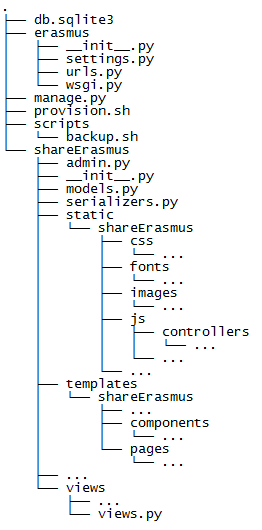
\includegraphics[width=5cm, keepaspectratio]{img/arbol.png}
  \caption{Esquema de ficheros del proyecto}
  \label{fig:arbol}
\end{figure}

Como se ha comentado anteriormente, cuando el servidor recibe una petición HTTP por parte del cliente, dicha petición es manejada desde el fichero \textit{urls.py}. Tras encontrar la url en este fichero, se hace ejecutar la función correspondiente del fichero \textit{views.py}. La función trata la petición GET y  responde con una respuesta HTTP que devuelve una plantilla \textit{HTML} al cliente.


\section{Diseño e implementación del servidor} 
\label{sec:diseno-servidor}

\subsection{Modelos de la base de datos} 
\label{subsec:modelo-base-datos}

La aplicación requiere de una base de datos donde se guarde información requerida para su correcto funcionamiento. La estructura de datos se guarda en el fichero \textit{models.py}. Django se encarga de generar las tablas pertinentes dentro de la base de datos. La base de datos utilizada en esta aplicación es \textit{SQLite3}.
\newline

A continuación se enumeran y describen cada uno de los modelos creados para la aplicación web, así como los campos de cada uno de ellos:

\begin{itemize}
    \item \textbf{Asignatura:} modelo que representa una asignatura en una universidad. El nombre de una asignatura es único solamente dentro de una universidad (otra universidad puede tener una asignatura con ese mismo nombre). Los campos del modelo son:
    \begin{itemize}
        \item \textbf{Nombre:} nombre de la asignatura.
        \item \textbf{Universidad:} referencia a la universidad donde se imparte la asignatura.
        \item \textbf{Descripción:} descripción de la asignatura, donde se incluye la dificultad, el modelo de evaluación, tipo de exámenes, de prácticas, etc.
        \item \textbf{Convalidaciones:} información relativa a las asignaturas que se convalidan.
        \item \textbf{Créditos ECTS:} número de créditos ECTS de la asignatura.
    \end{itemize}

    \item \textbf{Universidad:} modelo que representa una universidad. Los campos del modelo son:
    \begin{itemize}
        \item \textbf{Nombre:} nombre de la universidad.
        \item \textbf{Ciudad:} referencia a la ciudad a la que pertenece la universidad.
        \item \textbf{Descripción:} descripción general de la universidad, donde pueden describirse los edificios universitarios tales como la biblioteca, la cafetería, los aularios, los laboratorios, etc.
        \item \textbf{Contactos:} comentarios que aporten información para poder contactar con la universidad de destino.
        \item \textbf{Latitud:} coordenada de la latitud en la que se encuentra la universidad.
        \item \textbf{Longitud:} coordenada de la longitud en la que se encuentra la universidad.
    \end{itemize}

    \item \textbf{Ciudad:} modelo que representa una ciudad. En él aparecen distintos campos en los que se guarda información de la ciudad dividida en diferentes categorías. Los campos del modelo son:
    \begin{itemize}
        \item \textbf{Nombre:} nombre de la ciudad.
        \item \textbf{País:} referencia al país al que pertenece la ciudad.
        \item \textbf{Descripción:} descripción general de la ciudad.
        \item \textbf{Alojamiento:} información relativa a dónde alojarse en la ciudad.
        \item \textbf{Transporte:} información relativa al transporte en la ciudad.
        \item \textbf{Precios:} información relativa a los precios generales de la vida en la ciudad.
        \item \textbf{Telefonía móvil:} información relativa a las compañias telefónicas recomendadas.
        \item \textbf{Clima:} información relativa al clima en la ciudad.
        \item \textbf{Vida estudiantil:} información relativa al estilo de vida en la ciudad.
        \item \textbf{Vida nocturna:} información relativa a lugares de salida nocturna recomendados.
        \item \textbf{Cuenta bancaria:} información relativa a los bancos recomendados para abrir una cuenta, sacar dinero, etc.
        \item \textbf{Restaurantes:} información relativa a restaurantes o bares donde comer.
        \item \textbf{Compras:} información relativa a los lugares para comprar en la ciudad.
        \item \textbf{Cultura:} información relativa a lugares y monumentos de la ciudad.
        \item \textbf{Turismo:} información relativa a otras ciudades cercanas recomendadas para visitar.
        \item \textbf{Otra información:} otra información de la ciudad que no encaje en ninguno de los campos anteriores.
    \end{itemize}
    \item \textbf{País:} modelo que representa un país. El campo del modelo es:
     \begin{itemize}
        \item \textbf{Nombre:} nombre del país.
    \end{itemize}
    \item \textbf{Perfil de usuario:} modelo que representa a un usuario. Es un modelo que hereda los campos del modelo User de \textit{Django}. Los campos importantes heredados son:
     \begin{itemize}
        \item \textbf{Nombre de usuario:} nombre de usuario. Debe ser único. Será el identificador utilizado para iniciar sesión.
        \item \textbf{Correo electrónico:} correo electrónico del usuario. Debe ser único.
        \item \textbf{Contraseña:} contraseña de la cuenta del usuario.
        \item \textbf{Nombre:} nombre del usuario.
        \item \textbf{Apellidos:} apellidos del usuario.
    \end{itemize}
Además, se han añadido los siguientes campos:
    \begin{itemize}
        \item \textbf{Correo electrónico público:} boolean que indica si se muestra o no el correo electrónico a los visitantes de la aplicación web.
        \item \textbf{Asignaturas:} referencia a las asignaturas cursadas por el usuario.
    \end{itemize}
    \item \textbf{Comentario:} modelo que representa un comentario realizado sobre una universidad o sobre una asignatura. Los campos del modelo son:
    \begin{itemize}
        \item \textbf{Usuario:} referencia al perfil de usuario que realiza el comentario.
        \item \textbf{Cuerpo:} contenido del comentario.
        \item \textbf{Fecha:} día y hora en el que se realizó el comentario.
        \item \textbf{Universidad:} referencia a la universidad donde se ha escrito el comentario. Es posible que este campo no contenga ninguna referencia.
        \item \textbf{Asignatura:} referencia a la asignatura donde se ha escrito el comentario.  Es posible que este campo no tenga ninguna referencia.
    \end{itemize}
\end{itemize}


\subsection{API} 
\label{subsec:api}

Se ha creado una API REST que permite el acceso a los datos de la base de datos a través de una interfaz web. De esta manera se consigue reducir en parte la carga computacional del servidor, ya que cada vez que se carga una página, el servidor no se encarga de insertar los datos de la base de datos en la plantilla, sino que esto se realiza desde el lado del cliente con funciones \textit{Javascript} que realizan peticiones a la API. 
\newline

La API también es la encargada de gestionar las peticiones POST que realizan los clientes al enviar un formulario desde las páginas de configuración que se describen en la sección \ref{subsec:vistas-configuracion}. Las peticiones POST se gestionan desde el fichero \textit{api.py}.
\newline

Los path de la API son:

\begin{itemize}
        \item \textbf{api/1.0/countries/:} contiene la información referida a los países.
        \item \textbf{api/1.0/countries/\textit{(id-country)}/:} contiene la información referida al país \textit{id-country}.
        \item \textbf{api/1.0/cities/:} contiene la información referida a las ciudades.
        \item \textbf{api/1.0/cities/\textit{(id-city)}/:} contiene la información referida a la ciudad \textit{id-city}.
        \item \textbf{api/1.0/universities/:} contiene la información referida a las universidades.
        \item \textbf{api/1.0/universities/\textit{(id-university)}/:} contiene la información referida a la universidad \textit{id-university}.
        \item \textbf{api/1.0/users/:} contiene la información referida a los usuarios.
        \item \textbf{api/1.0/users/\textit{(id-user)}/:} contiene la información referida al usuario \textit{id-user}.
        \item \textbf{api/1.0/subjects/:} contiene  la información referida a las asignaturas.
        \item \textbf{api/1.0/subjects/\textit{(id-subject)}/:} contiene  la información referida a la asignatura \textit{id-subject}.
        \item \textbf{api/1.0/comments/:} contiene  la información referida a los comentarios.
        \item \textbf{api/1.0/comments/\textit{(id-comment)}/:} contiene  la información referida al comentario \textit{id-comment}.
\end{itemize}

\subsection{Backups} 
\label{subsec:backups}

Un elemento importante que no puede faltar en una aplicación de estas características es el \textit{backup}. Tratándose de una aplicación web \textbf{colaborativa}, es necesario realizar múltiples copias de seguridad de la base de datos ya que hay mucha información que puede ser modificada por cualquier usuario, pudiendo hacer borrados menores o incluso masivos. De esta manera se pretende evitar la pérdida de información que pudieran ocasionar usuarios maliciosos, o símplemente despistados. 
\newline

Para hacer copias de la base de datos automáticamente se utiliza una herramienta de \textit{Linux} llamada \textit{cron}, la cual permite ejecutar tareas repetitivas periódicamente. En este caso el  \textit{script} que se quiere ejecutar es \textit{backup.sh}. Para ello~\cite{pagina-crontab} es necesario editar el fichero \textit{/etc/crontab} (Ver Figura~\ref{fig:crontab}) y añadir al final la siguiente línea: 

\verb|0 3 * * * root sh /tfg/tfg/scripts/backup.sh|. El archivo de \textit{crontab} tiene la siguiente estructura de izquierda a derecha: Minutos (rango de 0-59), Horas (0-23), Día del mes (1-31), Mes (1-12), Día de la semana (0-6 siendo 0=Domingo), Path completo al \textit{script} o programa que queramos ejecutar.

\begin{figure}[H]
  \centering
  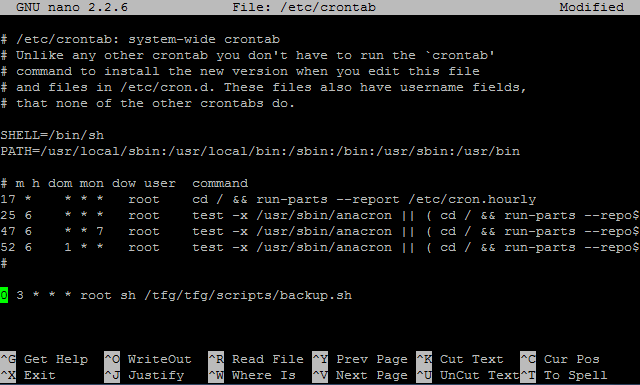
\includegraphics[width=14cm, keepaspectratio]{img/crontab.png}
  \caption{Archivo /etc/crontab}
  \label{fig:crontab}
\end{figure}

En el  \textit{script} mencionado anteriormente se ejecutan los comandos necesarios para hacer copias de la base de datos. Para no saturar el servidor, se realiza una copia cada día, y se almacena durante una semana. Así se evita que una gran cantidad de copias de la base de datos pueda ocupar demasiado espacio en el servidor pudiendo colapsarlo. Por lo tanto siempre hay 7 copias correspondientes a los últimos 7 días, y en el momento en el que se detectara algún borrado se sustituiría la base de datos por una de las guardadas anteriormente.



\section{Diseño e implementación del cliente} 
\label{sec:diseno-cliente}

El cliente puede acceder a la interfaz de la aplicación a través de un navegador web. Como se ha comentado en la sección \ref{sec:tecnologias-web}, para el desarrollo del lado del cliente se han utilizado las tecnologías  \textit{HTML5},  \textit{CSS3} y  \textit{Javascript}. Las dos primeras son necesarias para definir cómo se visualizan y con qué estilos y diseño cada uno de los elementos visibles en la aplicación, como puede ser la barra del menú superior, el listado de las universidades, los comentarios, etc.  \textit{Javascript}, y más concretamente el  \textit{framework Angular JS}, se utiliza para gestionar el flujo de información de la parte del cliente. Esto es posible con la utilización de los controladores de  \textit{Angular JS}. Así es posible incluir en las vistas de la aplicación web los datos obtenidos de la base de datos a través de peticiones a la API.
\newline

En cuanto a la interfaz, se ha utilizado la plantilla \textit{Margo}~\cite{pagina-margo}. La plantilla se ha adaptado a las necesidades propias de la aplicación y se han  creado nuevos elementos y estilos para hacerla más atractiva. Entre las características que se han añadido ha sido la creación de usuarios, algo que no contempla la plantilla original.

{\large  \textbf{Interfaz para dispositivos móviles}\par}

La interfaz de usuario utiliza la técnica \textit{Responsive Design}, lo que permite que se adapte a cualquier tipo de pantalla y dispositivos de cualquier tamaño.

\subsection{Vistas de las páginas} 
\label{subsec:vistas-paginas}

A continuación se describen una a una todas las páginas de la aplicación, explicando cada elemento que aparece en las páginas, así como su utilidad. Todas las páginas son públicas y accesibles para todo tipo de usuarios, tanto para usuarios registrados como para los no registrados.
\newline

En todas las páginas aparece una barra superior, a través de la cual se puede acceder de manera sencilla a la página de inicio, la página de universidades, la página de ayuda y a la página de contacto. Además, si el usuario no está registrado, aparece un enlace hacia la página de inicio de sesión y registro, y si el usuario está registrado, los enlaces se corresponden con la página de perfil del usuario, las distintas páginas de configuración (que se detallan en la sección \ref{subsec:vistas-configuracion}) y un enlace para cerrar la sesión.
\newline

{\large  \textbf{Página de inicio}\par}

En la vista de inicio\footnote{url relativa:\url{/}} se hace un resumen de las características que tiene la aplicación web para hacer más fácil la navegación a través de ella (ver Figura~\ref{fig:inicio}).
\newline

\begin{figure}[H]
  \centering
  
\includegraphics[width=14cm, keepaspectratio]{img/inicio.png}
  \caption{Página de inicio}
  \label{fig:inicio}
\end{figure}

{\large  \textbf{Página de inicio de sesión y registro}\par}

La vista de inicio de sesión y registro\footnote{url relativa:\url{/sign}} está dividida en dos partes (ver Figura~\ref{fig:inicio-sesion-registro}). En el lado derecho aparece un formulario que permite registrar a un nuevo usuario de una manera rápida, y en el lado izquierdo está el formulario para iniciar sesión con una cuenta registrada anteriormente.
\newline

\begin{figure}[H]
  \centering
  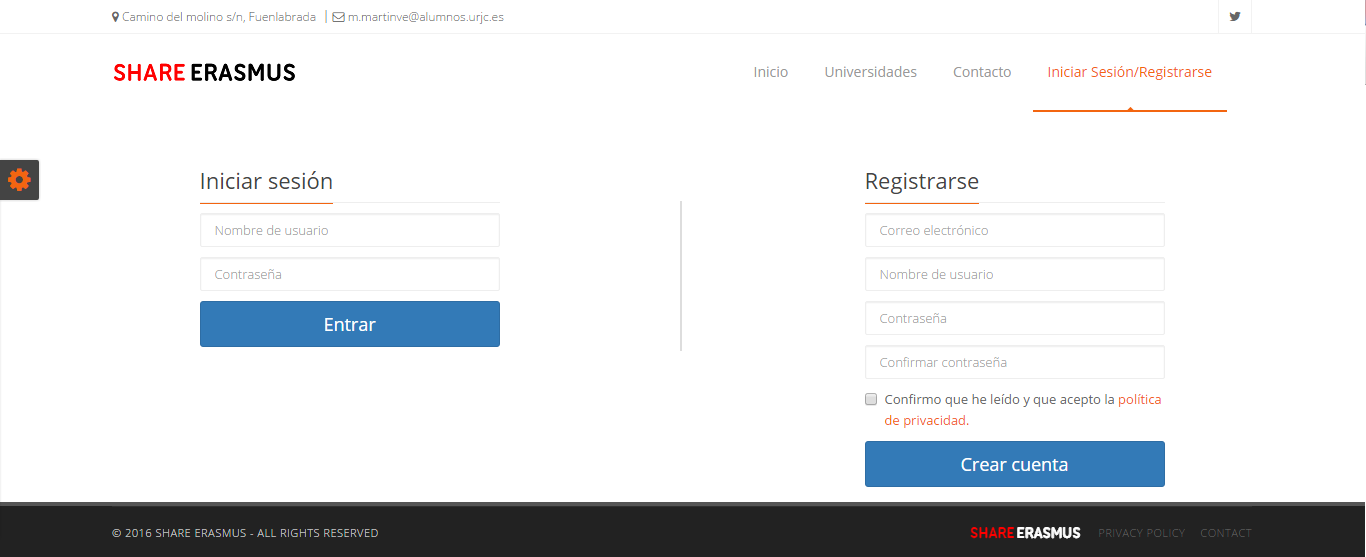
\includegraphics[width=16cm, keepaspectratio]{img/inicio-sesion-registro.png}
  \caption{Página de inicio de sesión y registro}
  \label{fig:inicio-sesion-registro}
\end{figure}

En el formulario de registro se requiere que el usuario introduzca su cuenta de correo electrónico, un nombre de usuario y la contraseña. Además, se pide que se lea y acepte la política de privacidad. El correo electrónico no es público para el resto de personas a no ser que el propio usuario así lo indique. El correo electrónico puede hacerse público en la página de configuración de la cuenta.
\newline

La autenticación en la aplicación se realiza a través del formulario de inicio de sesión. El identificador para iniciar sesión es el nombre de usuario, que irá acompañado de su correspondiente contraseña. 
\newline

{\large  \textbf{Página de universidades}\par}

En esta vista\footnote{url relativa:\url{/universities}} se muestra un listado de todas las universidades añadidas por los usuarios registrados en la aplicación (Ver Figura~\ref{fig:universidades}).
\newline

Lo primero que cabe destacar de esta vista es el buscador superior. Se trata de una búsqueda predictiva. Al introducir un texto, aparecen todos los resultados de universidades que contienen la cadena de texto introducida. Esto se realiza con la librería  \textit{angucomplete-alt}~\cite{pagina-angucomplete} de  \textit{Angular JS}, cuya función es buscar a través de la API las coincidencias entre el texto introducido en el buscador y los nombres de las universidades guardadas en la base de datos. Debajo de este buscador se muestra un enlace a través del cual, sólo si el usuario está registrado, se accede a la página de configuración donde se puede crear una nueva universidad.
\newline

\begin{figure}[H]
  \centering
  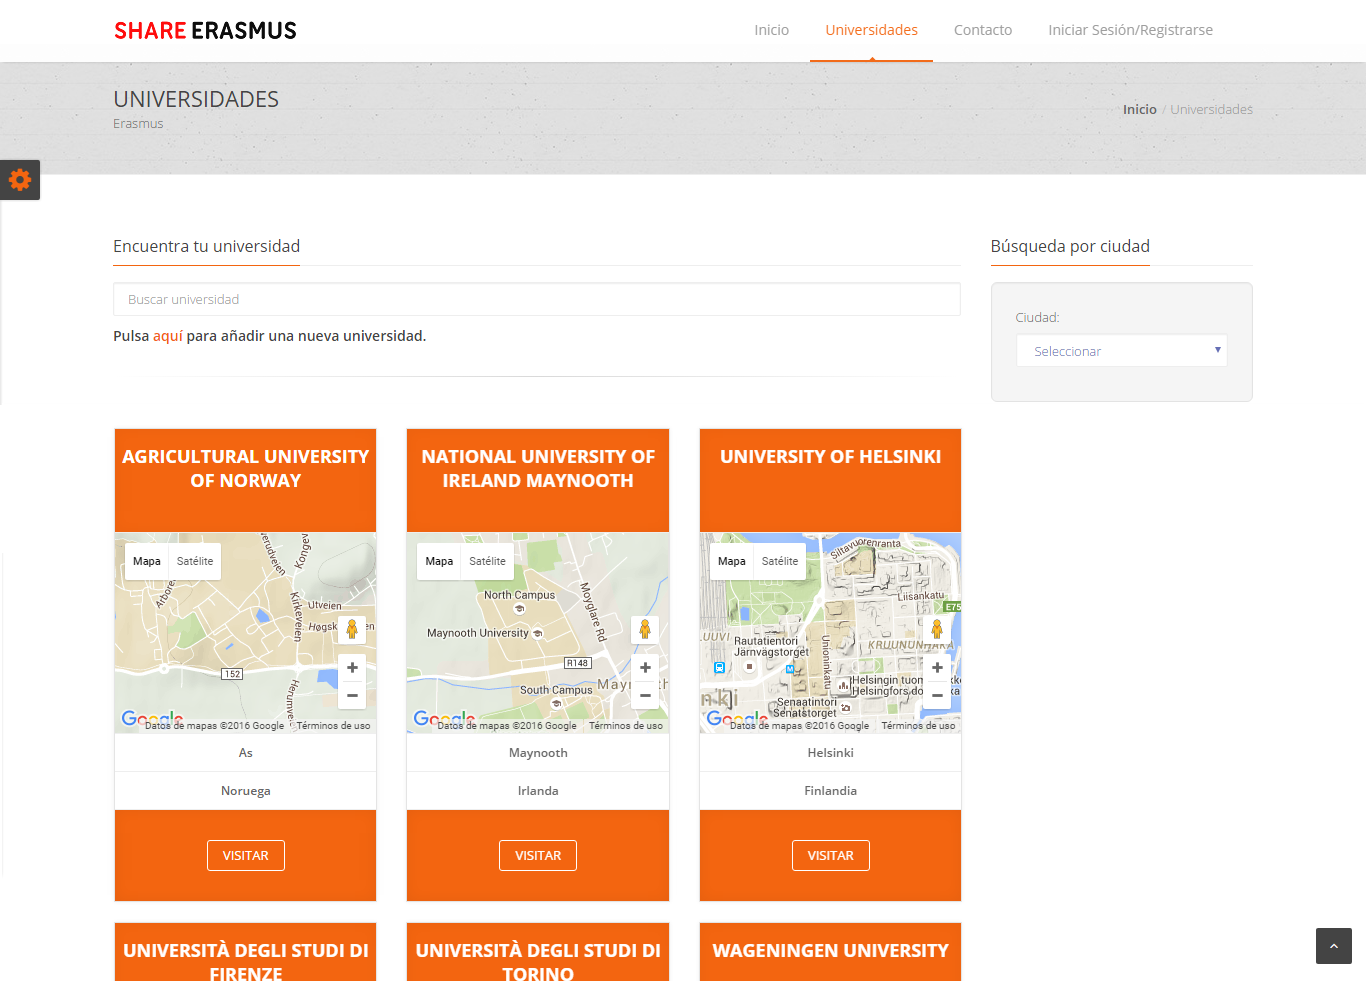
\includegraphics[width=14cm, keepaspectratio]{img/universidades.png}
  \caption{Página de universidades}
  \label{fig:universidades}
\end{figure} 

En la parte central de la vista se muestra una lista de todas las universidades, distribuidas en filas de tres en tres y ordenadas alfabéticamente. De cada universidad se muestra su nombre, un mapa de Google Maps\footnote{\url{https://developers.google.com/maps/documentation/geocoding/intro}} que muestra su localización, el nombre de la ciudad de la universidad y su país. Además a través del botón \textit{VISITAR} se accece a la página de esa universidad.
\newline

En la parte de la derecha se muestra un filtro que permite mostrar únicamente todas las universidades que se localicen en la ciudad seleccionada.
\newline

Tras haber realizado un filtrado, debajo del buscador superior aparece un botón que permite volver a mostrar el listado de todas las universidades.

{\large  \textbf{Página de una universidad}\par}

En esta vista\footnote{url relativa:\url{/universities/(id-university)}} se muestra información relativa a la universidad y a su ciudad (Ver Figura~\ref{fig:universidad}). La información relativa a la universidad la pueden añadir los usuarios desde la página de configuración de mis universidades, y la relativa a la ciudad desde la página de configuración de mis ciudades.


\begin{figure}[H]
  \centering
  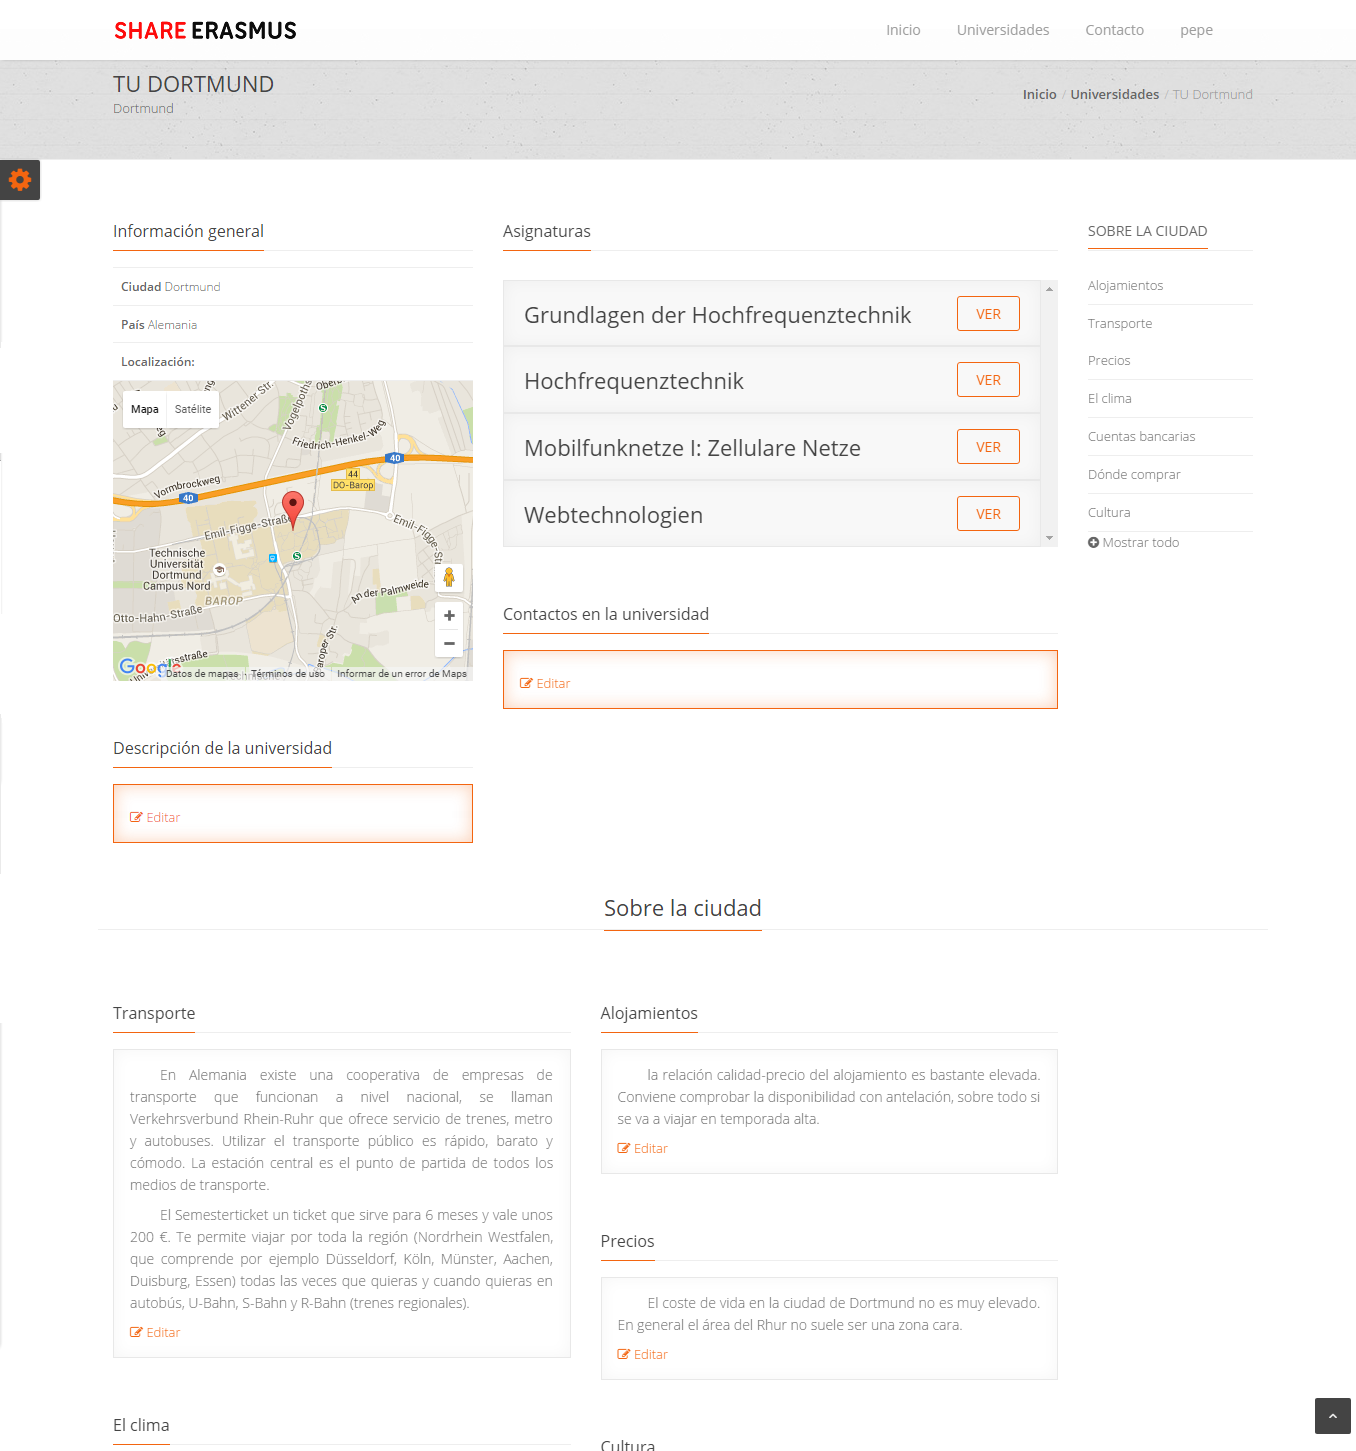
\includegraphics[width=16cm, keepaspectratio]{img/universidad.png}
  \caption{Página de una universidad}
  \label{fig:universidad}
\end{figure}

En la parte superior izquierda se visualiza la información general de la universidad, como es el nombre de su ciudad y su país, además de mostrar un mapa de Google con su localización.
\newline

En la parte superior central se muestra un listado de todas las asignaturas que se imparten en la universidad. A través del botón \textit{VER} de cada una de ellas se accede a la página de esa asignatura.
\newline

Justo debajo de la información general de la universidad y del listado de asignaturas se muestra distinta información relativa a la universidad.
\newline

En el lateral derecho de la vista se muestra un listado de las distintas categorías con información relativa a la ciudad. Al pulsar sobre cualquiera de ellas se accede directamente a visualizar la información sobre esa categoría. Al final de la listas de categorías hay un botón que al pulsarlo muestra la lista completa de categorías, tanto las que tienen información como las que no. Toda la información relativa a la ciudad se muestra en esta vista debajo de la información relativa a la universidad. 
\newline

Por último, debajo de toda la información de la ciudad aparecen comentarios que pueden realizar los usuarios. Solo pueden comentar usuarios registrados, aunque los comentarios son visibles por cualquier visitante de la página.

{\large  \textbf{Página de una asignatura}\par}

En esta vista\footnote{url relativa:\url{/universities/(id-university)/(id-subject)}} (Ver Figura~\ref{fig:contacto}) se muestra información relativa a una asignatura. Esta información puede ser añadida por los usuarios desde la página de configuración de mis asignaturas.
\newline

A la izquierda se muestra el número de créditos ETCS de los que consta la asignatura, una descripción e información relativa a las convalidaciones de las asignaturas.
\newline

A la derecha aparece un listado de los usuarios que han seleccionado la asignatura desde la página de configuración de mis universidades. Al pulsar sobre el nombre de un alumno se accede a la página de perfil de ese usuario.
\newline

\begin{figure}[H]
  \centering
  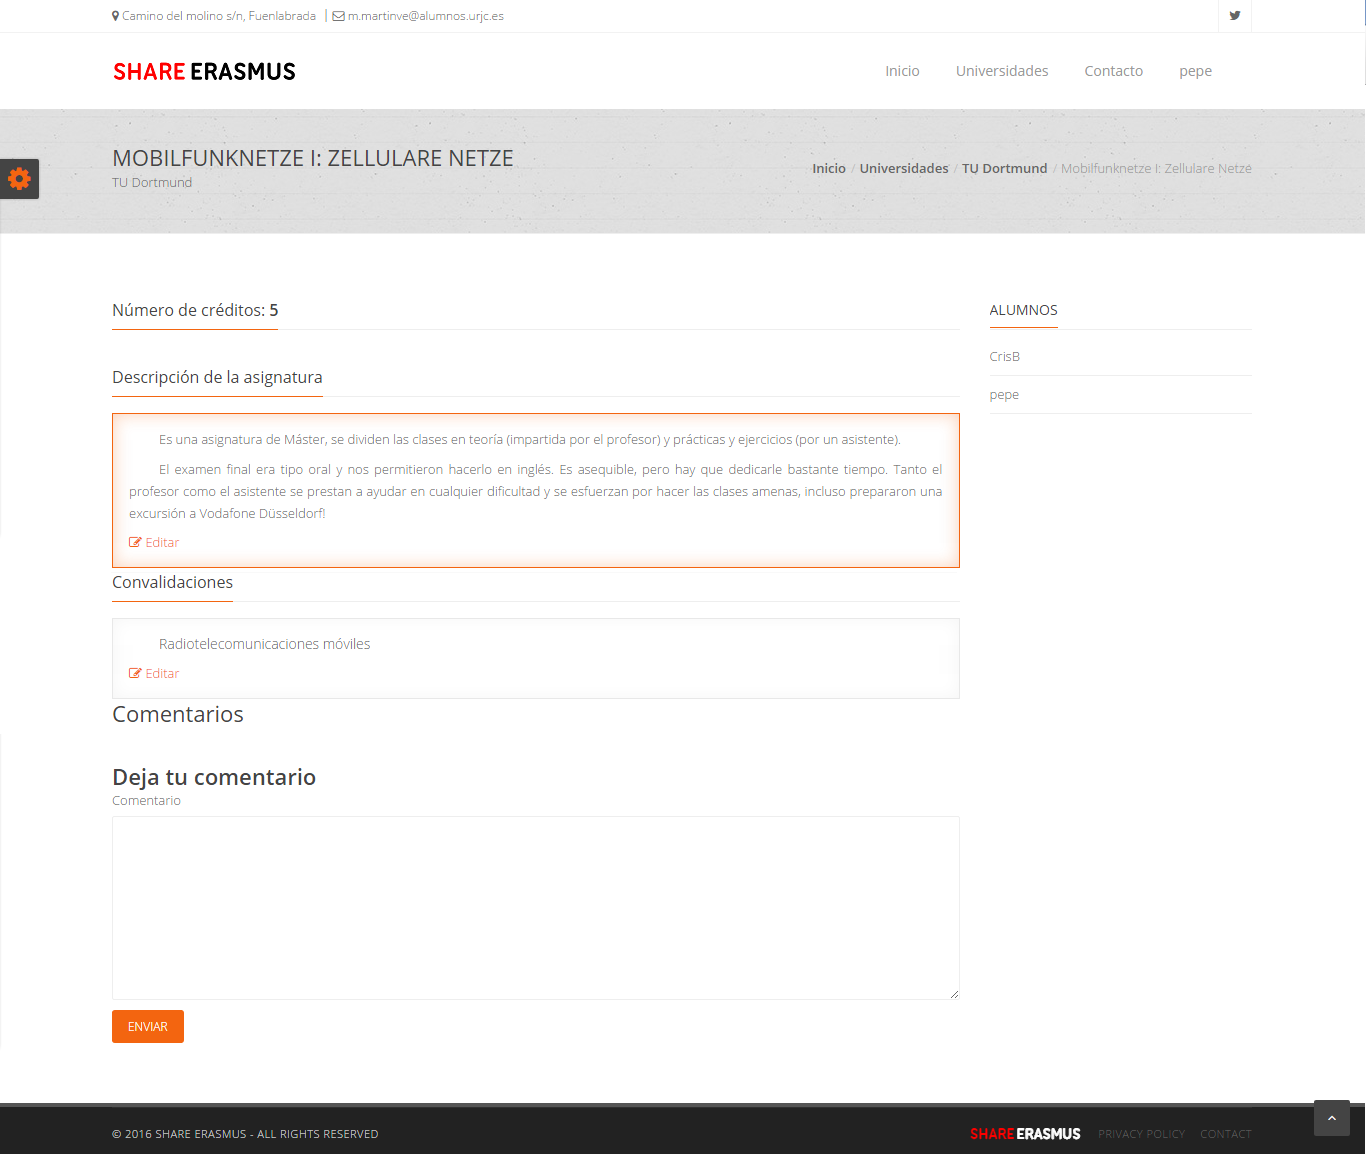
\includegraphics[width=14cm, keepaspectratio]{img/asignatura.png}
  \caption{Página de una asignatura}
  \label{fig:asignatura}
\end{figure}

Por último, al igual que en la página de una asignatura, debajo de la información de la asignatura aparecen comentarios realizados por los usuarios.

{\large  \textbf{Página de perfil de un usuario}\par}

En esta vista\footnote{url relativa:\url{/users/(username)}} se muestra información sobre un usuario (Ver Figura~\ref{fig:perfil-usuario}).
\newline

Se muestra una barra en la parte superior de la página donde aparece el nombre del usuario y un enlace a la página de inicio. Más abajo se muestra una imagen de perfil. Además, si el usuario permite que se muestre su correo electrónico, aparecerá junto al nombre completo del
\begin{figure}[H]
  \centering
  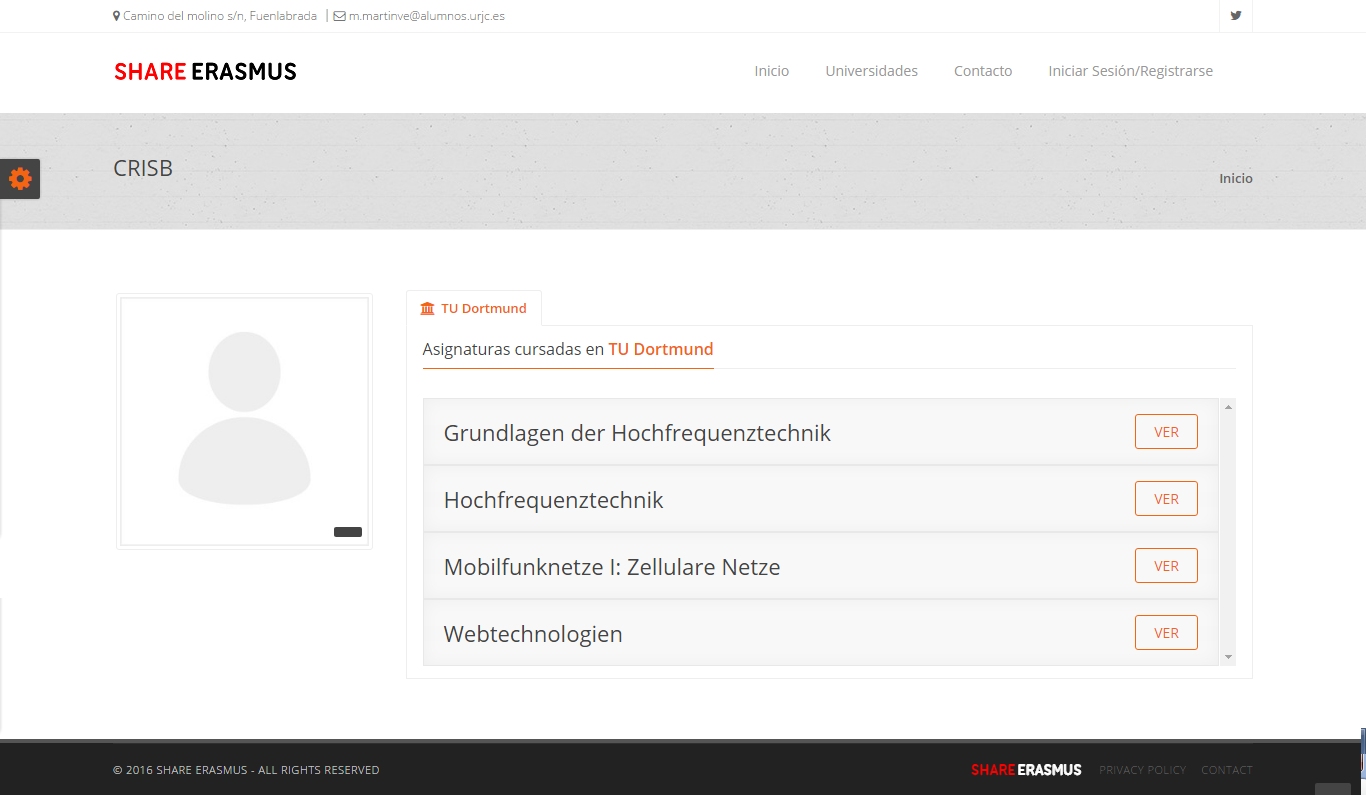
\includegraphics[width=16cm, keepaspectratio]{img/perfil-usuario.png}
  \caption{Página de un usuario}
  \label{fig:perfil-usuario}
\end{figure} usuario (si ha proporcionado la información en la página de configuración de la cuenta).
\newline

A la derecha se muestran las universidades donde el usuario ha indicado que ha estudiado o tiene intención de estudiar. Al pulsar sobre el nombre de la universidad aparece una lista con las asignaturas cursadas o por cursar del usuario. Al pulsar en el botón \textit{VER} de una asignatura se accede a la página de esa asignatura.
\newline

{\large  \textbf{Página de contacto}\par}

A través de esta vista\footnote{url relativa:\url{/contact}} se puede contactar con el administrador de la aplicación para cualquier duda o sugerencia (Ver Figura~\ref{fig:contacto}).
\newline

\begin{figure}[H]
  \centering
  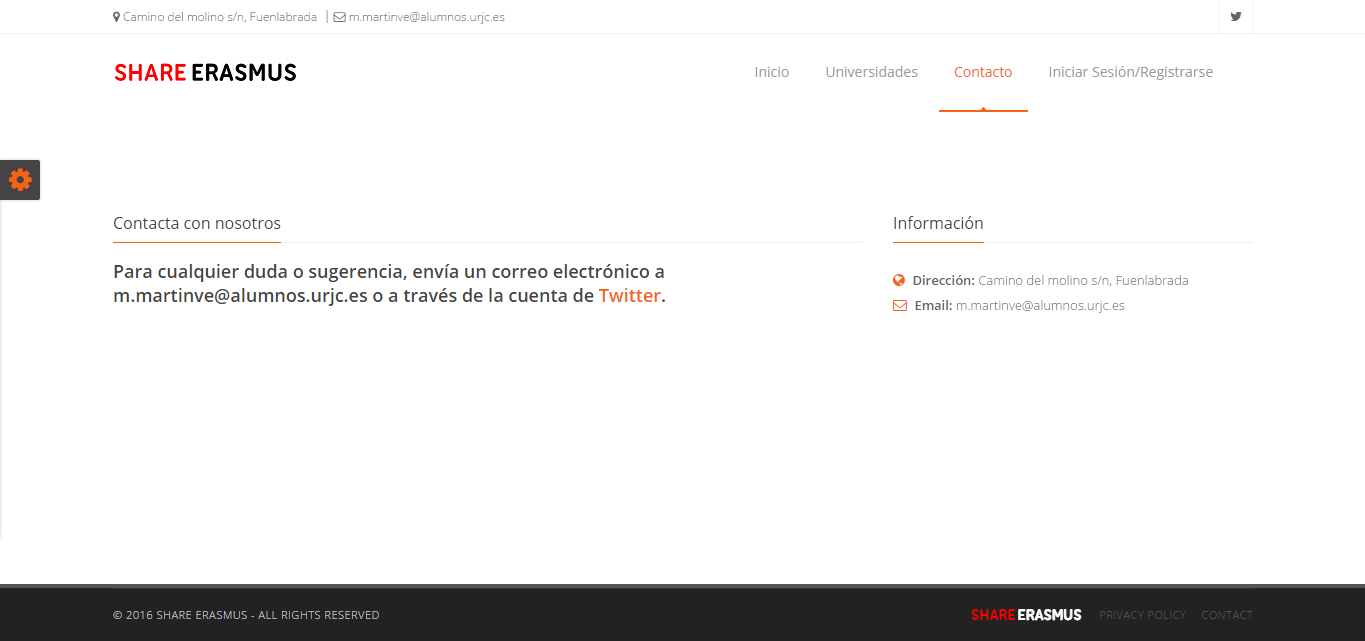
\includegraphics[width=16cm, keepaspectratio]{img/contacto.png}
  \caption{Página de contacto}
  \label{fig:contacto}
\end{figure}

{\large  \textbf{Página de política de privacidad}\par}

En esta vista\footnote{url relativa:\url{/privacy_policy}} se muestra información relativa a la información que se recopila y puede ser visible de los usuarios en esta aplicación (Ver Figura~\ref{fig:politica-privacidad}).

\begin{figure}[H]
  \centering
  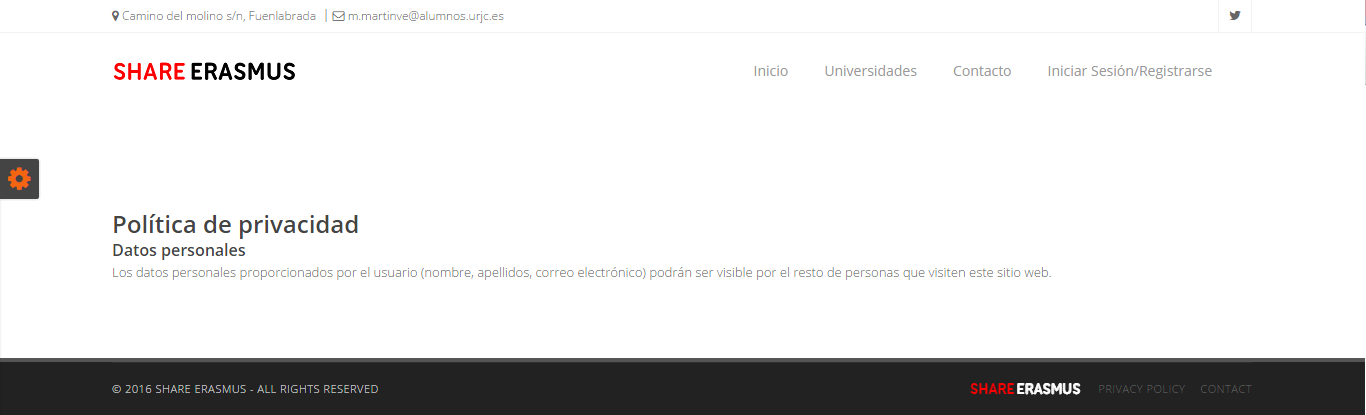
\includegraphics[width=16cm, keepaspectratio]{img/politica-privacidad.png}
  \caption{Página de política de privacidad}
  \label{fig:politica-privacidad}
\end{figure}

\subsection{Vistas de la configuración} 
\label{subsec:vistas-configuracion}

A continuación se describen las vistas de las páginas que son accesibles únicamente por usuarios registrados en la aplicación. Se puede acceder desde los enlaces que aparecen a la derecha en la barra superior. Desde estas vistas se completa tanto información personal del usuario como información relevante de las universidades, ciudades o asignaturas cursadas por el usuario.
\newline

Todas las vistas de configuración tienen un menú en el lateral izquierdo desde donde se puede acceder a los diferentes sitios de configuración.
\newline

{\large  \textbf{Página de configuración de mi cuenta}\par}

En esta vista\footnote{url relativa:\url{/settings/account}} aparece un formulario donde se pide al usuario (si lo desea) completar algunos datos personales (Ver Figura~\ref{fig:mi-cuenta}).
\newline

\begin{figure}[H]
  \centering
  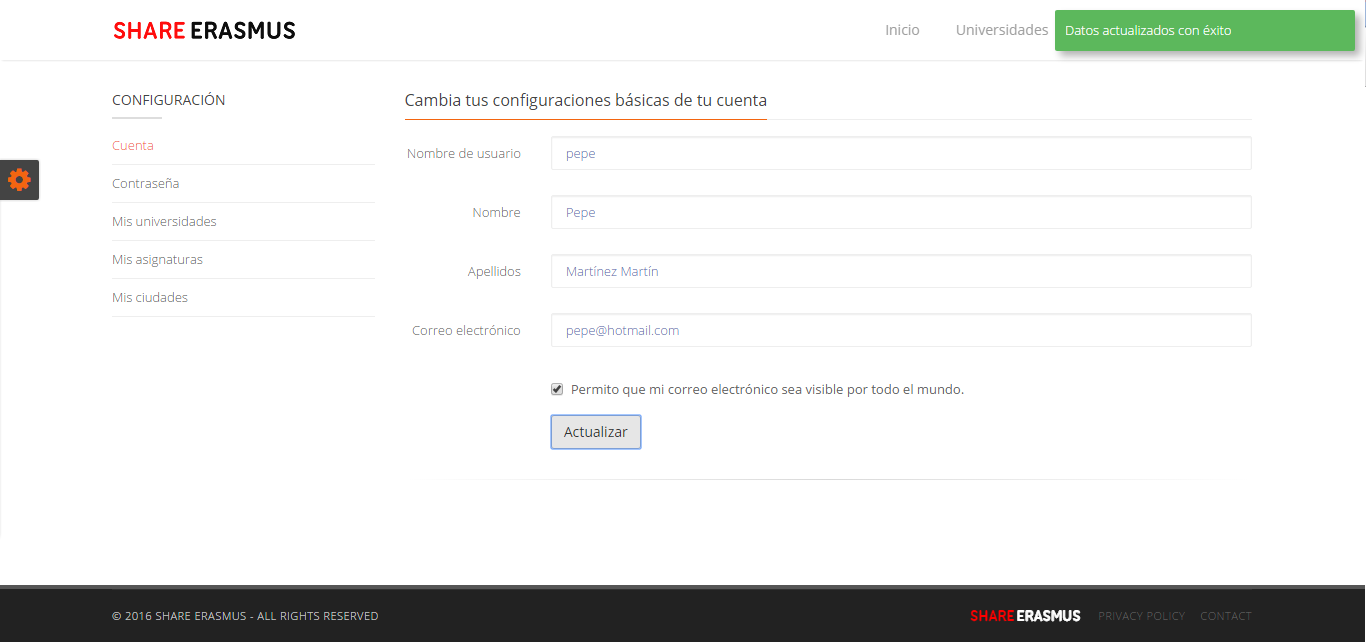
\includegraphics[width=16cm, keepaspectratio]{img/mi-cuenta.png}
  \caption{Página de configuración de la cuenta}
  \label{fig:mi-cuenta}
\end{figure}

Puede modificarse el nombre de usuario y el correo electrónico con los que el usuario se registró y añadir información como el nombre y los apellidos. Además aparece un \textit{checkbox} que puede marcarse si el usuario quiere que el correo electrónico pueda ser visible por cualquier persona que visite su página de perfil.
\newline

{\large  \textbf{Página de cambio de contraseña}\par}

En esta vista\footnote{url relativa:\url{/settings/password}} aparece un formulario donde se puede cambiar la contraseña de la cuenta (Ver Figura~\ref{fig:contrasena}). En el formulario se deben introducir la contraseña actual y la nueva contraseña.
\newline

\begin{figure}[H]
  \centering
  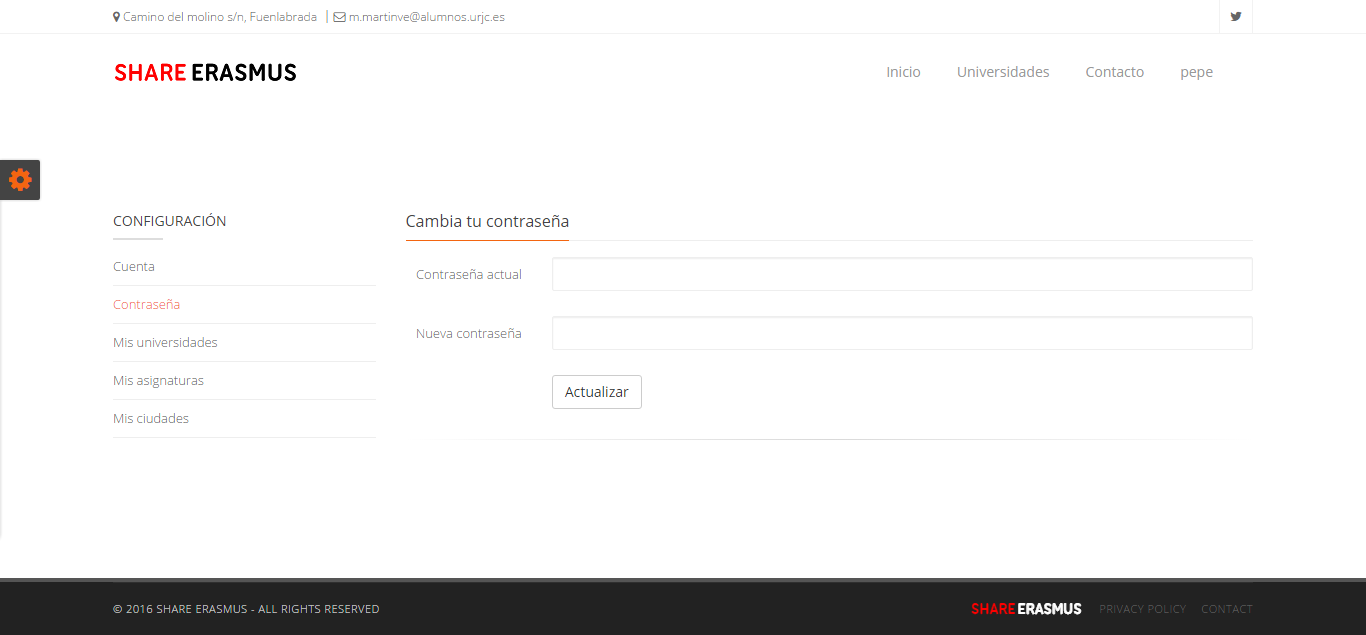
\includegraphics[width=16cm, keepaspectratio]{img/contrasena.png}
  \caption{Página de cambio de contraseña}
  \label{fig:contrasena}
\end{figure}

{\large  \textbf{Página de configuración de mis universidades}\par}

Desde esta vista\footnote{url relativa:\url{/settings/universities}} se pueden hacer dos funciones: buscar universidad y crear universidad. Lo primero que debe hacer un usuario cuando quiera registrarse en una universidad y en sus asignaturas cursadas o por cursar, es buscar la universidad en cuestión por si ya hubiera sido creada anteriormente.  (Ver Figura~\ref{fig:mis-universidades})
\newline

Al pulsar sobre \textit{Buscar universidad} aparecen varios filtros, que hay que utilizarlos en orden. En el primer filtro se debe seleccionar el país donde se encuentra la universidad, después se selecciona la ciudad y finalmente la universidad. A continuación se muestran algunas asignaturas que se imparten en dicha universidad, y el usuario debe seleccionar las que haya cursado o esté interesado en cursar. Además, si hay alguna asignatura que no aparezca en la lista, se pueden crear un máximo de 6 asignaturas a la vez. Al pulsar en \textit{Guardar} quedan registradas las asignaturas en la cuenta del usuario. 
\newline

\begin{figure}[H]
  \centering
  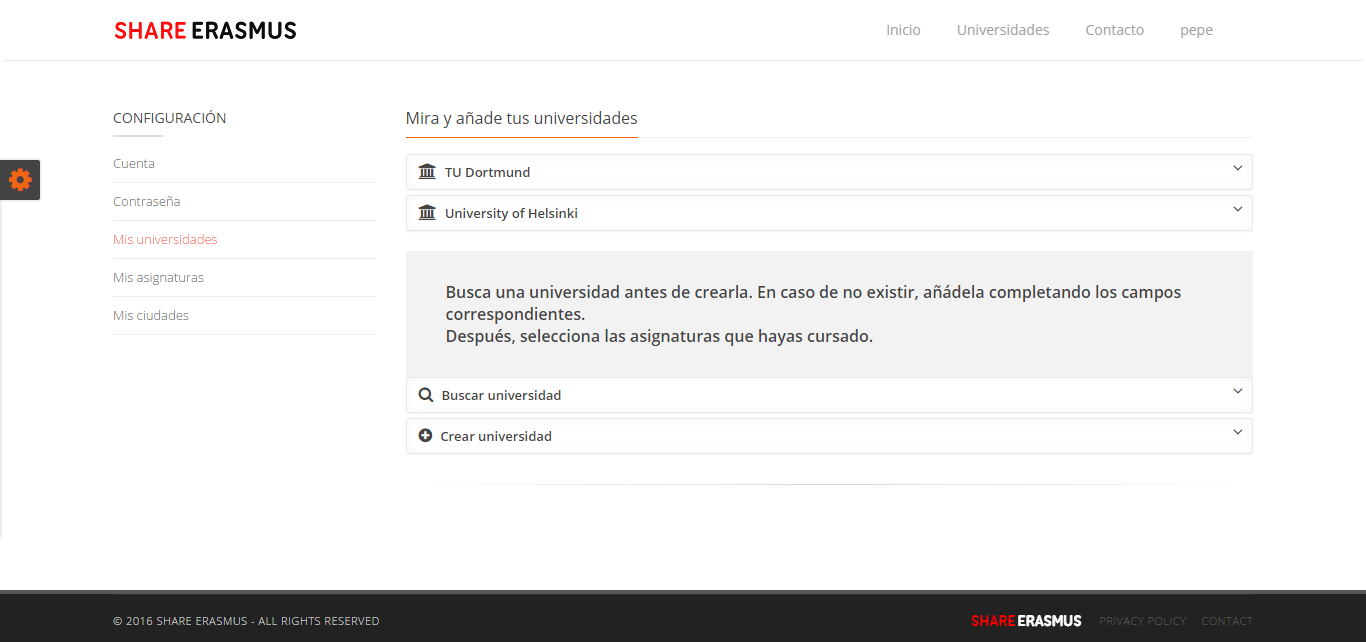
\includegraphics[width=16cm, keepaspectratio]{img/mis-universidades.png}
  \caption{Página de configuración de mis universidades}
  \label{fig:mis-universidades}
\end{figure}

Al recargar la página se muestra en la parte superior el nombre de la universidad. Al pulsar sobre él, aparece un formulario con varios campos de texto para completar información sobre la universidad: descripción y contactos (descritos en \ref{subsec:modelo-base-datos}). Al ser una aplicación web colaborativa, todos los usuarios registrados en una universidad puede modificar esa información. Se trata de complementar información que han escrito otros usuarios o añadir información nueva, tratando de que no se elimine información escrita por otros usuarios.
\newline

En caso de haber buscado una universidad y no haberla encontrado, existe la opción de crear una universidad. Al pulsar sobre \textit{Crear universidad} aparece un formulario en el que se debe introducir el nombre de la universidad, su ciudad y su país. Tras guardarla se debe recargar la página para buscar la universidad (de la manera descrita anteriormente) y seleccionar las asignaturas que sean oportunas.
\newline


{\large  \textbf{Página de configuración de mis asignaturas}\par}

En esta vista\footnote{url relativa:\url{/settings/subjects}} se muestra un listado de las asignaturas seleccionadas desde la vista de configuración de mis universidades (Ver Figura~\ref{fig:mis-asignaturas}). 
\newline

\begin{figure}[H]
  \centering
  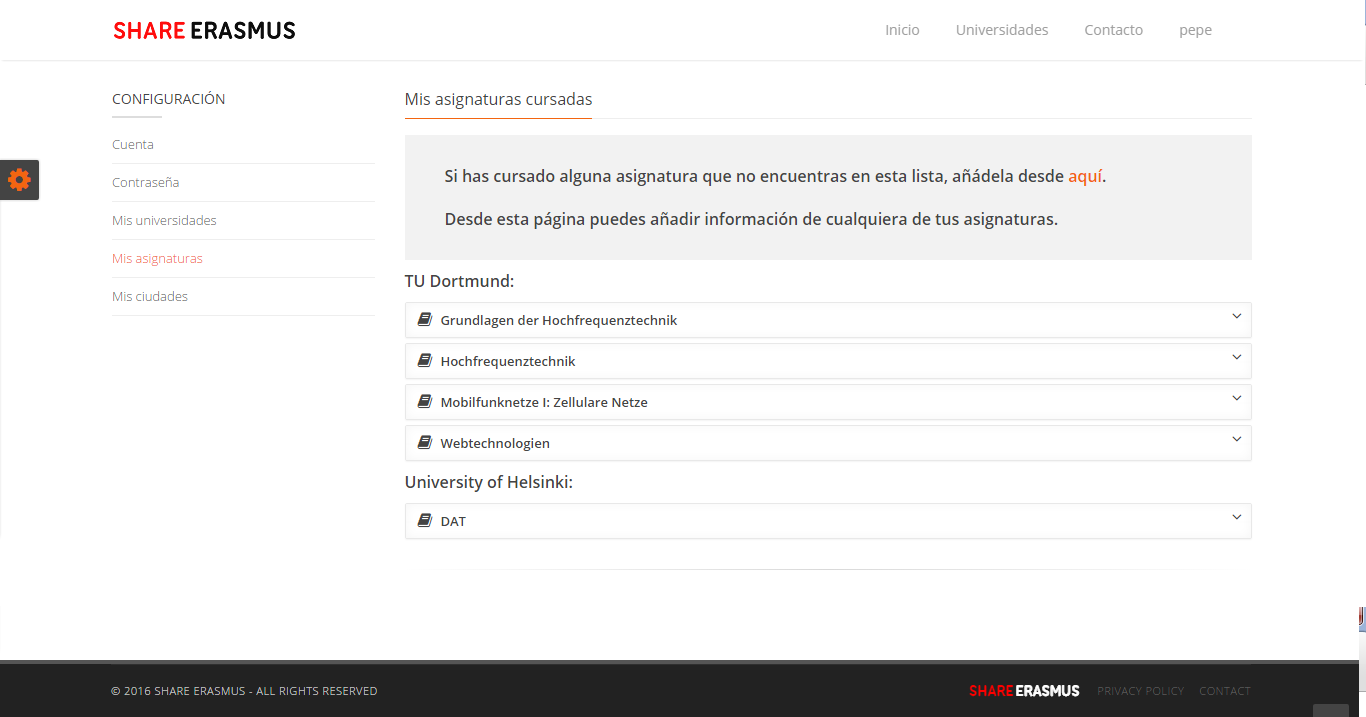
\includegraphics[width=16cm, keepaspectratio]{img/mis-asignaturas.png}
  \caption{Página de configuración de mis asignaturas}
  \label{fig:mis-asignaturas}
\end{figure}

Al pulsar sobre una de ellas se muestra un formulario para completar información sobre la asignatura. Esta información es la que aparece en la página de la asignatura.
\newline

 La información que puede añadirse es el número de créditos ECTS que se convalidan y una descripción, en la que se podría añadir información relativa a la dificultad de la asignatura, la forma de evaluación, tipo de exámenes, prácticas, etc. Es decir, cualquier información que otro usuario quisiera conocer antes de decidirse por escoger esa asignatura para sus estudios Erasmus.
\newline

{\large  \textbf{Página de configuración de mis ciudades}\par}

En esta vista\footnote{url relativa:\url{/settings/cities}} se muestra un listado de las ciudades donde el alumno ha estudiado, en el caso de ser en más de un lugar (Ver Figura~\ref{fig:mis-ciudades}). 
\newline

Al pulsar sobre el nombre de la ciudad se muestra un amplio formulario que permite completar información relativa a la ciudad. Esta información se muestra en la páginas de las universidades que pertenezcan a la ciudad.
\newline

\begin{figure}[H]
  \centering
  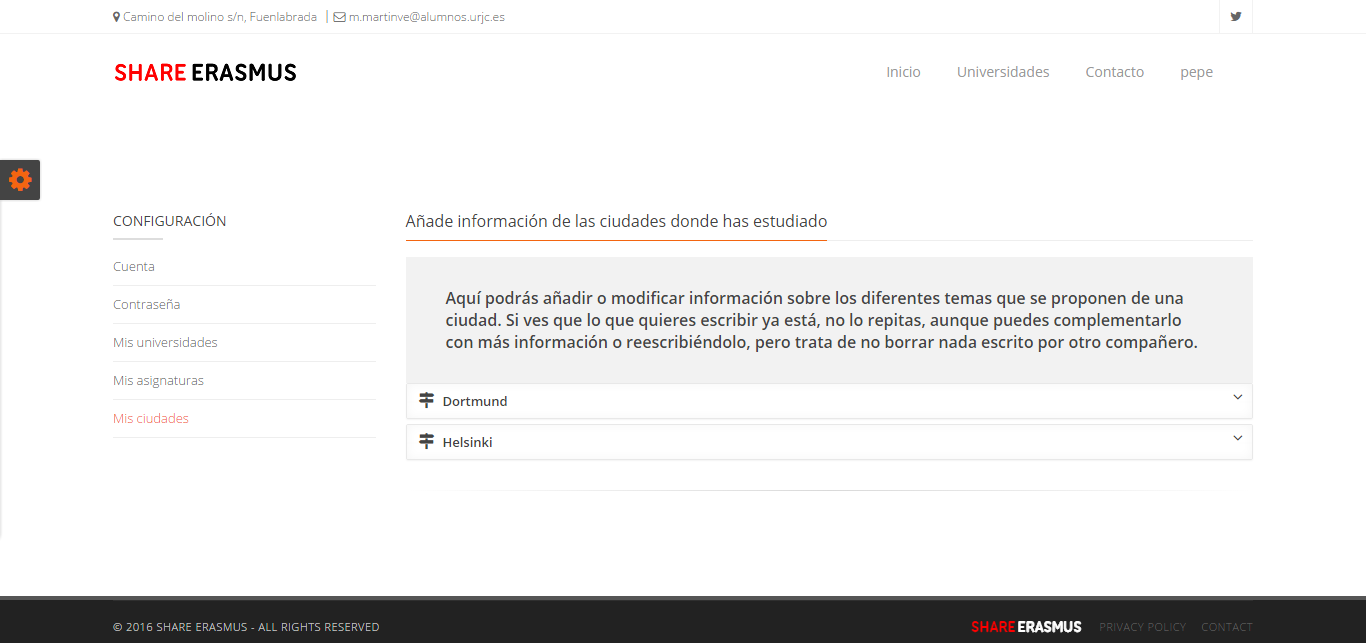
\includegraphics[width=16cm, keepaspectratio]{img/mis-ciudades.png}
  \caption{Página de configuración de mis ciudades}
  \label{fig:mis-ciudades}
\end{figure}

El formulario está dividido en diferentes categorías. No es necesario que el usuario rellene información de todas las categorías, aunque sí sería recomendable por el bien de la comunidad de la aplicación. Las diferentes categorías son: descripción de la ciudad, información sobre el alojamiento en la ciudad, el transporte, los precios, la telefonía móvil, la climatología, la vida de estudiante, la vida nocturna, bancos o cajeros, restaurantes o bares, \textit{shopping}, monumentos o lugares turísticos, lugares que visitar fuera de la ciudad y otra información relevante que no esté representada en ninguna categoría. Todas estas categorías están descritas en \ref{subsec:modelo-base-datos}.

\subsection{Vista del panel de administración} 
\label{subsec:vista-administrador}

Django ofrece unas vistas para administrar la base de datos que es muy útil y fácil de usar. Desde ahí se puede crear, modificar o eliminar cualquier elemento que se desee y hacer un seguimiento de la base de datos. En la Figura~\ref{fig:panel-administracion} se observa la vista principal del panel de administración.

\begin{figure}[H]
  \centering
  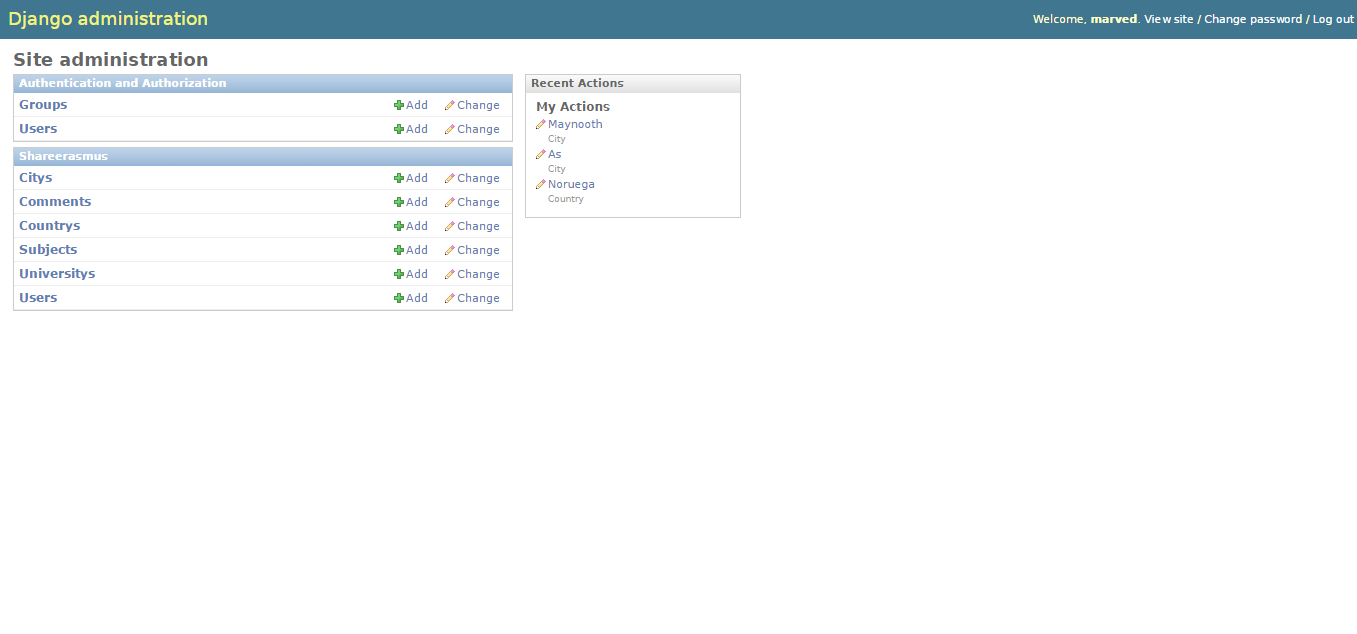
\includegraphics[width=16cm, keepaspectratio]{img/panel-administracion.png}
  \caption{Página de administración}
  \label{fig:panel-administracion}
\end{figure}

%%%%%%%%%%%%%%%%%%%%%%%%%%%%%%%%%%%%%%%%%%%%%%%%%%%%%%%%%%%%%%%%%%%%%%%%%%%%%%%%
%%%%%%%%%%%%%%%%%%%%%%%%%%%%%%%%%%%%%%%%%%%%%%%%%%%%%%%%%%%%%%%%%%%%%%%%%%%%%%%%
% RESULTADOS %
%%%%%%%%%%%%%%%%%%%%%%%%%%%%%%%%%%%%%%%%%%%%%%%%%%%%%%%%%%%%%%%%%%%%%%%%%%%%%%%%

\cleardoublepage
\chapter{Resultados}

A medida que se va desarrollando la aplicación web es necesario probar su funcionamiento con cada nueva funcionalidad añadida. Para ello se creó un entorno virtual de desarrollo con \textit{Vagrant}, ya que permite instalar y configurar software en una máquina virtual que simula estar en el servidor en el que se alojará la aplicación web.
\newline

Una vez que la aplicación ya estaba bastante avanzada, se procedió a desplegarla en un servidor remoto. Se contrató el servicio de alojamiento web que ofrece OVH. De esta manera la aplicación ya podía ser utilizada por los usuarios.
\newline

Fue importante el momento en el que se hizo el despliegue en el servidor remoto ya que permitió que visitaran la web algunas personas que colaboraron con sus ideas en la mejora de la aplicación. 
\newline

Todas las pruebas de funcionalidad de la aplicación se han realizado en un entorno local (preproducción), y una vez que se comprobaba que todo funcionaba correctamente se procedía a introducir los cambios en el servidor remoto (producción).


\section{Pruebas en servidor local} 
\label{sec:pruebas-en-servidor-local}

Como se ha comentado anteriormente, se ha utilizado \textit{Vagrant} para crear un entorno virtual de desarrollo. Para ello ha sido necesario instalar \textit{VirtualBox}\footnote{\url{https://www.virtualbox.org/wiki/Downloads}} y \textit{Vagrant}\footnote{\url{https://www.vagrantup.com/downloads.html}}. También ha sido necesario instalar en la máquina virtual\textit{ Django}, \textit{Git} y los diferentes paquetes y librerías necesarias para el correcto funcionamiento de la aplicación web. Así, se ha creado el archivo de instalación \textit{provision.sh}.
\newline

Una vez instalado todo lo necesario, para ejecutar la máquina virtual es necesario introducir en una \textit{Shell Unix}: \begin{verbatim} 
$vagrant up 
$vagrant provision
\end{verbatim}  

 Para probar la aplicación web desde el navegador hay que introducir una url que contenga la dirección IP y el puerto configurados en el archivo \textit{Vagrantfile} de esta forma: \textit{http://IP:PUERTO/}.
\newline

Y para apagar la máquina se ejecuta la siguiente instrucción:
\begin{verbatim} 
$vagrant halt 
\end{verbatim}  

En este entorno es en el que se han ido probando todas las funcionalidades nuevas que se han ido desarrollando, lo que ha permitido corregir errores y revertirlos.

\section{Pruebas en servidor remoto} 
\label{sec:pruebas-en-servidor-remoto}

Se ha contratado un servidor VPS en la web de OVH, que ofrece un buen rendimiento y seguridad. Además ha sido necesario contratar un dominio a través del cual los usuarios pudieran acceder a la aplicación web. El dominio elegido ha sido \url{shareerasmus.com}.
\newline

Tras accdeder mediante \textit{ssh} a la máquina virtual contratada, lo primero que ha sido necesario hacer es clonar el repositorio \textit{Git}\footnote{\url{https://github.com/marved/tfg}} (donde está el trabajo alojado) en la máquina virtual, para posteriormente ejecutar el archivo \textit{provision.sh}. 
\newline

Tras tener todo el entorno instalado, para ejecutar la aplicación se necesita ejecutar en la \textit{Shell Unix} el comando:
\begin{verbatim} 
$python manage.py runserver shareerasmus.com:80
\end{verbatim}  

Como se ha comentado anteriormente, aquí solo se despliega la aplicación cuando ha sido revisada desde el entorno local y se ha comprobado que las nuevas funcionalidades que se han ido desarrollando funcionan correctamente. Las pruebas en este entorno las realizan los usuarios informando de posibles errores o aconsejando mejoras que pudieran hacerse para mejorar la experiencia en la navegación a través de la web.

\section{Resultado final} 
\label{sec:resultado-final}

El resultado final es satisfactorio. Se ha conseguido desplegar la aplicación tanto en el servidor local como en uno remoto, pudiendo ser accesible para todos los usuarios que visitaran la página \url{shareerasmus.com}. Se han ido solventando, con mayores o con menores problemas todos los \textit{bugs} que han ido apareciendo, y aunque sería mejorable la velocidad de navegación, se ha consiguido una aplicación web útil para la comunidad Erasmus y fácilmente navegable.




%%%%%%%%%%%%%%%%%%%%%%%%%%%%%%%%%%%%%%%%%%%%%%%%%%%%%%%%%%%%%%%%%%%%%%%%%%%%%%%%
%%%%%%%%%%%%%%%%%%%%%%%%%%%%%%%%%%%%%%%%%%%%%%%%%%%%%%%%%%%%%%%%%%%%%%%%%%%%%%%%
% CONCLUSIONES %
%%%%%%%%%%%%%%%%%%%%%%%%%%%%%%%%%%%%%%%%%%%%%%%%%%%%%%%%%%%%%%%%%%%%%%%%%%%%%%%%

\cleardoublepage
\chapter{Conclusiones}
\label{chap:conclusiones}


\section{Consecución de objetivos}
\label{sec:consecucion-objetivos}

Este trabajo pretendía crear una aplicación web colaborativa que fuera útil para futuros alumnos Erasmus. La aplicación debía proporcionar información relevante que hiciera más fácil a los estudiantes elegir el destino europeo preferido. Y la aplicación tiene la capacidad de contener toda esa información bien organizada y dividida en distintas categorías. 
\newline

A continuación se enumeran los objetivos específicos que se han conseguido y los que se han quedado incompletos:

\begin{itemize}
        \item \textbf{Estudiar las necesidades de los estudiantes:} se ha contactado con varios alumnos y alumnas que han disfrutado de una beca Erasmus, ya sean de la ETSIT o no, que han colaborado para conseguir que la temática de la información contenida en la aplicación resulte útil para los futuros estudiantes Erasmus.
        \item \textbf{Uso de tecnologías web avanzadas:} se han utilizado varias tecnologías web. Las que más cabe destacar son las mencionadas varias veces en anteriores capítulos, como son \textit{HTML5}, \textit{CSS3}, \textit{Angular JS} y \textit{Django}. Todas ellas han facilitado el desarrollo de esta aplicación web gracias a sus grandes funcionalidades y características, consiguiendo un buen resultado final.
        \item \textbf{Web colaborativa:} Toda la información que se puede encontrar en la aplicación ha sido creada por los usuarios que la han utilizado. No ha habido muchos usuarios, pero si se consiguiera que el número se incrementara, podría ser una web muy útil para todos los futuros estudiantes Erasmus de la ETSIT.
        \item \textbf{Sencillez en su uso:} se ha realizado una interfaz bastante sencilla e intuitiva, para que la experiencia de navegación de los usuarios sea lo más cómoda posible. Además, en las páginas de configuración se han escrito comentarios para que los usuarios tengan claro lo que significa cada formulario y desde dónde hay que realizar cada función que se quiera hacer.
        \item \textbf{Web social:} se ha conseguido que los usuarios puedan aportar información a la aplicación sobre las universidades, las ciudades y las asignaturas. Además se ha aportado un mecanismo de interactuación entre usuarios por medio de comentarios tanto en la página de cada universidad como en la página de cada asignatura. Sin embargo no se han llegado a crear otros mecanismos como pudieran ser foros o mensajes directos entre usuarios, que permitieran una mayor fluidez en la comunicación entre ellos.
        \item \textbf{Copias de seguridad:} se ha conseguido crear copias de seguridad de la base de datos. Para evitar sobrecargar el servidor, las copias duran como máximo una semana. De esta manera siempre habría 7 copias de la base de datos correspondientes a los últimos 7 días.
        \item \textbf{Migrar el proyecto a un servidor remoto:} se ha alojado la aplicación en un servidor remoto para permitir de una forma sencilla que pudiera ser visitada por otras personas.
\end{itemize}


\section{Aplicación de lo aprendido}
\label{sec:aplicacion}


\begin{enumerate}
  \item \textbf{Fundamentos de la programación:} la primera asignatura de programación de la carrera, donde se aprenden los primeros conceptos básicos de programación. El lenguaje utilizado en esta asignatura fue \textit{Ada}, un lenguaje que no he aplicado en el desarrollo de este proyecto, pero que sirvió para comenzar a aprender a programar.
  \item \textbf{Sistemas telemáticos y Arquitectura de redes de ordenadores:} han sido útiles porque aprendí el funcionamiento de los protocolos y peticiones HTTP, algo fundamental cuando se desarrolla una aplicación web.
  \item \textbf{Servicios y aplicaciones telemáticas:} en esta asignatura desarrollé mi primera aplicación web con el \textit{framework Django}. Ha sido de gran ayuda ya que la parte de la gestión del servidor de este proyecto está basada en \textit{Django}.
  \item \textbf{Ingeniería de sistemas de información:} en esta asignatura comencé a utilizar el lenguaje \textit{Javascript}. Fue una primera toma de contacto con el lenguaje.
  \item \textbf{Desarrollo de aplicaciones telemáticas:} en esta asignatura terminé de adquirir las capacidades necesarias para poder realizar el lado del cliente con el lenguaje \textit{Javascript}. Con los conocimientos adquiridos en la anterior asignatura, en esta los apliqué y aprendí más sobre sobre la programación web en el lado del cliente. Además aprendí a utilizar distintas \textit{APIs} como la de Google que he utilizado en este proyecto.
  
\end{enumerate}


\section{Lecciones aprendidas}
\label{sec:lecciones_aprendidas}

 He aprendido a desarrollar un proyecto de gran envergadura como lo es éste, y a desarrollar mis capacidades de trabajo y superación, resolviendo los problemas con los que me he ido encontrando. He conseguido fortalecer gran parte de los conocimientos aprendidos en las asignaturas de programación o telemática de la carrera.
\newline

Sobre todo he fortalecido los conocimientos de \textit{HTML5}, \textit{CSS3}, \textit{Javascript}, \textit{Django} y peticiones HTTP. Además he aprendido a utilizar más a fondo un \textit{framework} tan útil para el desarrollo web como es \textit{Angular JS}, que empecé a utilizar realizando unas prácticas laborales y me ha permitido desarrollar el \textit{backend} de la aplicación de una manera bastante sencilla.
\newline

Y no menos importante, para la redacción de esta memoria ha sido muy útil haber aprendido a redactar con \textit{LaTex}\footnote{https://www.latex-project.org/}, que a pesar de que puede resultar bastante incómodo, es imprescindible utilizarlo para conseguir una buena presentación formal de la memoria de este TFG.



\section{Trabajos futuros}
\label{sec:trabajos_futuros}

\begin{itemize}
  \item \textbf{Más social:} las aplicaciones y páginas web están en continua evolución hacia un modelo lo más social posible. Se busca la mejor comunicación posible entre los usuarios. Por ello, una línea de trabajo futuro sería la creación de un foro, posibilidad de enviar mensajes directos entre usuarios y la creación de un chat que permita una comunicación más dinámica entre usuarios.
  \item \textbf{Ampliar a más universidades:} esta versión de la aplicación está orientada únicamente para alumnos de una misma universidad. Sería interesante ampliar el \textit{target} de la aplicación y que estuviera orientado a alumnos de todo tipo de universidades y carreras, incluyendo universidades de toda Europa que forman parte del programa Erasmus.
  \item \textbf{Multilenguaje:} debido al multilenguaje europeo, debería traducirse la aplicación a distintos idiomas, como mínimo al inglés.
  \item \textbf{Mejor eficiencia:} siempre puede mejorarse la eficiencia de la aplicación, y debería mejorarse sobre todo las peticiones a la base de datos para así tener una mayor velocidad de navegación.
  \item \textbf{Aplicación móvil:} una aplicación móvil que ofrezca todas las funcionalidades que ofrece la aplicación web. El móvil es muy utilizado entre los jóvenes, y una aplicación móvil sería muy útil.
  \item \textbf{Administración:} sería interesante crear un panel de administración más elaborado que el que proporciona \textit{Dango}, que además incluyera la posibilidad de que, debido a que el contenido de la aplicación es generado por los usuarios, un moderador recibiera avisos cuando algún campo de la base de datos haya sido modificado y pudiera revisarlo y controlar que no se escribe nada inoportuno o fuera de lugar.
\end{itemize}


%%%%%%%%%%%%%%%%%%%%%%%%%%%%%%%%%%%%%%%%%%%%%%%%%%%%%%%%%%%%%%%%%%%%%%%%%%%%%%%%
%%%%%%%%%%%%%%%%%%%%%%%%%%%%%%%%%%%%%%%%%%%%%%%%%%%%%%%%%%%%%%%%%%%%%%%%%%%%%%%%
% BIBLIOGRAFIA %
%%%%%%%%%%%%%%%%%%%%%%%%%%%%%%%%%%%%%%%%%%%%%%%%%%%%%%%%%%%%%%%%%%%%%%%%%%%%%%%%

\cleardoublepage

% Las siguientes dos instrucciones es todo lo que necesitas
% para incluir las citas en la memoria
\bibliographystyle{unsrt}
\bibliography{memoria}  % memoria.bib es el nombre del fichero que contiene
% las referencias bibliogr�ficas. Abre ese fichero y mira el formato que tiene,
% que se conoce como BibTeX. Hay muchos sitios que exportan referencias en
% formato BibTeX. Prueba a buscar en http://scholar.google.com por referencias
% y ver�s que lo puedes hacer de manera sencilla.
% M�s informaci�n: 
% http://texblog.org/2014/04/22/using-google-scholar-to-download-bibtex-citations/


%%%%%%%%%%%%%%%%%%%%%%%%%%%%%%%%%%%%%%%%%%%%%%%%%%%%%%%%%%%%%%%%%%%%%%%%%%%%%%%%
%%%%%%%%%%%%%%%%%%%%%%%%%%%%%%%%%%%%%%%%%%%%%%%%%%%%%%%%%%%%%%%%%%%%%%%%%%%%%%%%
% APENDICE(S) %
%%%%%%%%%%%%%%%%%%%%%%%%%%%%%%%%%%%%%%%%%%%%%%%%%%%%%%%%%%%%%%%%%%%%%%%%%%%%%%%%

\cleardoublepage
\appendix
\chapter{Instalación y uso}
\label{app:instalacion-y-uso}

Para el correcto funcionamiento de la aplicación, lo primero que hay que hacer es ejecutar el archivo \textit{provision.sh}, para que se instalen todos los paquetes que son necesarios, si es que no están ya instalados en la máquina.

Una vez instalados, ejecutar en una \textit{Shell Unix} el comando \verb|python manage.py syncdb|, que creará una base de datos. A continuación hay que ejecutar un comando de la forma 

\verb|python manage.py runserver IP:PUERTO|, indicando una dirección IP y un puerto libre: \verb|python manage.py runserver localhost:8000|.

Cuando la aplicación esté en funcionamiento, habrá que introducir en un navegador la \textit{url} \textit{http://localhost:8000}


\chapter{Recurso para descargar la aplicación}
\label{app:descargar-aplicacion}

La aplicación web está disponible en el siguiente repositorio de \textit{Github}: 

\url{https://github.com/marved/tfg}




\end{document}
